\lstdefinelanguage{BibTeX}
{
    keywords={%
        @article,@book,@collectedbook,@conference,@electronic,@ieeetranbstctl,%
        @inbook,@incollectedbook,@incollection,@injournal,@inproceedings,%
        @manual,@mastersthesis,@misc,@patent,@periodical,@phdthesis,@preamble,%
        @proceedings,@standard,@string,@techreport,@unpublished%
    },
    comment=[l][\itshape]{@comment},
    sensitive=false,
}

\definecolor{codegreen}{rgb}{0,0.6,0}
\definecolor{codegray}{rgb}{0.5,0.5,0.5}
\definecolor{codepurple}{rgb}{0.58,0,0.82}
\definecolor{backcolour}{rgb}{0.95,0.95,0.92}

\lstdefinestyle{mystyle}{
    backgroundcolor=\color{backcolour},   
    commentstyle=\color{codegreen},
    keywordstyle=\color{magenta},
    numberstyle=\tiny\color{codegray},
    stringstyle=\color{codepurple},
    basicstyle=\ttfamily\tiny,
    breakatwhitespace=false,         
    breaklines=true,                 
    captionpos=b,                    
    keepspaces=true,                 
    numbers=left,                    
    numbersep=5pt,                  
    showspaces=false,                
    showstringspaces=false,
    showtabs=false,                  
    tabsize=2
}


\chapter{{\LaTeX} Tutorial}
\pagebreak

\begin{center}
{\LARGE\textbf{\LaTeX\ Tutorial}}
\end{center}

% ============================================================
\section{Using Lists}
\label{sec:using_lists}
% ============================================================

There are many ways to creating a list. In this section we show some of the most common examples and uses of lists. Remember, the sky is the limit.

\subsubsection{Simple Bullet Point List}

For simple bullet points you use \verb|itemize| within a begin and end tags. 

\begin{itemize}
    \item first item.
    \item second item.
    \item third item.
\end{itemize}

\subsubsection{Bullet Point List With Different Symbols}

We can change the bullet symbol as wee need by defining the symbol we use for each item.

\begin{itemize}     
    \item[\textbullet] first item.
    \item[$\square$] second item.
    \item[$-$] third item.
\end{itemize}

\subsubsection{Numbered List}

If we want to have a numbered list we use the \verb|\begin{enumerate}| \verb|...| \verb|\end{enumerate}| keyword to have a list like the one shown below.

\begin{enumerate}
    \item first item.
    \item second item.
    \item third item.
\end{enumerate}

\subsubsection{Custom Numbered List}

We can define the list numbering as we want. For example, sometimes we need to have a list of specific type like in the requirements gathering step. Hence, we say the first item should be named \emph{REQ-1}, and the second should be \emph{REQ-2} and so on. To get such numbered list we define a custom label as we need given the example below. 

\begin{enumerate}[label=\textbf{REQ-\arabic*:}]
    \item first item.
    \item second item.
    \item third item.
\end{enumerate}

\subsubsection{Items Spacing}

We can change the spacing between the symbol and the text and between each item as we want by changing the values of the \verb|noitemsep|, \verb|topsep|, \verb|parsep|, and \verb|partopsep|. 

\textcolor{red}{Note: we do not recommend changing the margin of anything as this template is designed to take care of all the formatting settings. You really need to have a good reason to change the margins.}

\begin{itemize}[noitemsep,topsep=10pt,parsep=10pt,partopsep=10pt]
\item item 1
\item item 2
\item item 3
\end{itemize}


% ============================================================
\section{Dealing with Figures}
\label{sec:dealing_with_figures}
% ============================================================

A figure is any content wrapped between \verb|\begin{figure}| and \verb|\end{figure}|. A figure (or any floating object) can have different options. However, we think the most important one that we should share with you is the positioning option of the figure. Each figure can be placed somewhere in a page by adding the position option after the begin keyword \verb|\begin{figure}[h]|. The list of positioning options and there meaning are given in Table-\ref{tab:position-options}.

\begin{table}[h!]
    \centering
    \begin{tabular}{p{0.15\textwidth}p{0.8\textwidth}}
        \hline\hline
        \textbf{Parameter} & \textbf{Position}                                                                                                            \\ \hline\hline
        h                  & Place the float here, i.e., approximately at the same point it occurs in the source text (however, not exactly at the spot)  \\ \hline
        t                  & Position at the top of the page.                                                                                             \\ \hline
        b                  & Position at the bottom of the page.                                                                                          \\ \hline
        p                  & Put on a special page for floats only.                                                                                       \\ \hline
        !                  & Override internal parameters {\LaTeX} uses for determining ``good'' float positions.                                            \\ \hline
        H                  & Places the float at precisely the location in the {\LaTeX} code. Requires the float package. This is somewhat equivalent to h!. \\ \hline\hline
    \end{tabular}
    \caption{Floating objects (e.g., figure) positioning options and their meanings.}
    \label{tab:position-options}
\end{table}


\subsection{Simple Figure}

Adding a figure simply require you to point {\LaTeX} to the image/pdf file location inside a \verb|\begin{figure}| \verb|...| \verb|\end{figure}| environment. The figure below (Figure-\ref{ref:simple-figure}) include an image in a file located in \verb|figures/samples/earth-in-space.jpg|. We do not resize the image or change any of its attributes. Also, we use the option \verb|H| to place the figure right after this text.


\begin{figure}[H]
    \begin{center}
        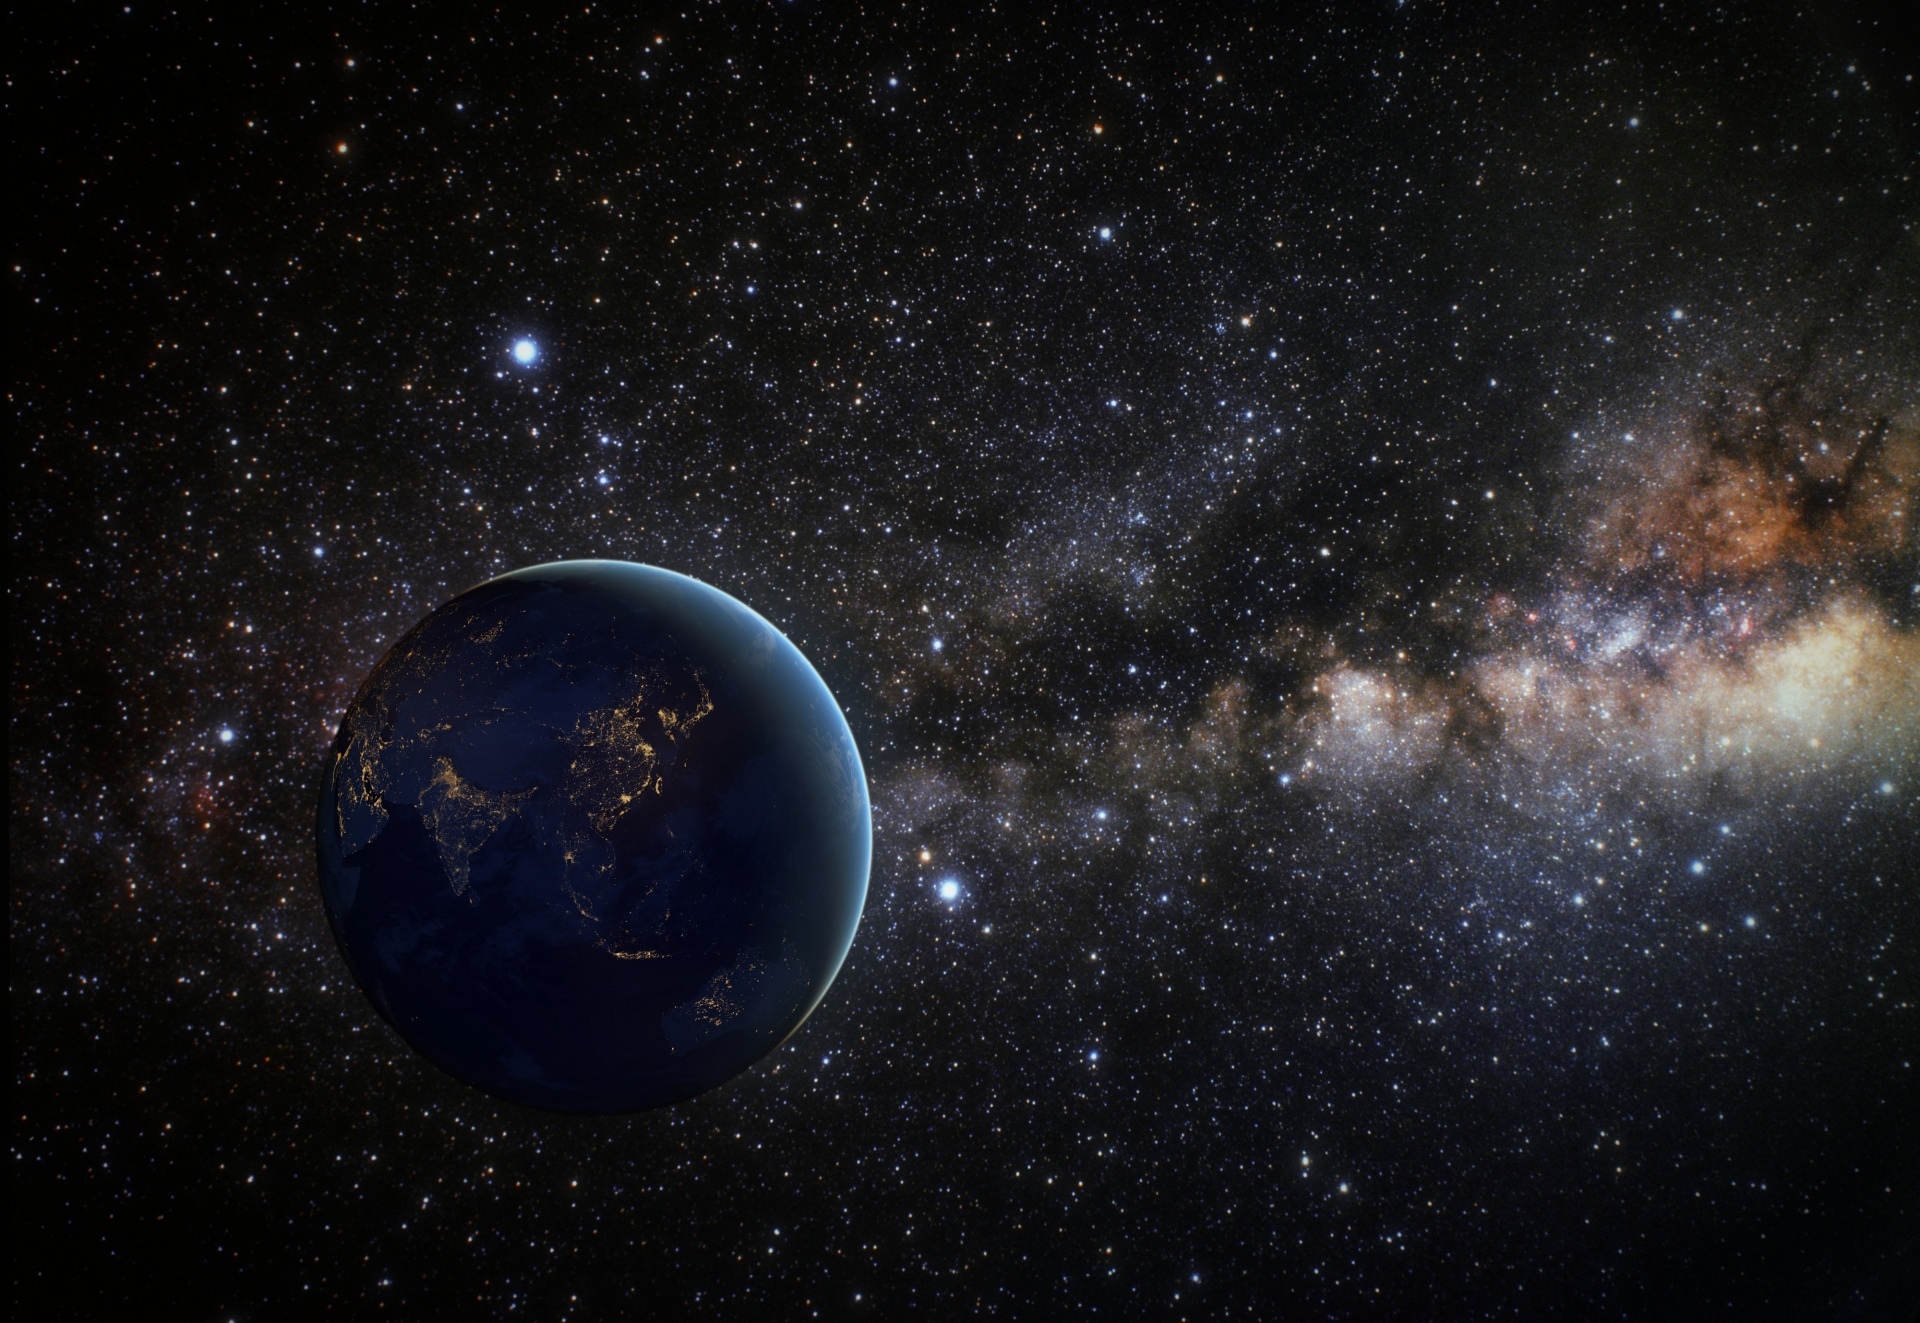
\includegraphics{figures/samples/earth-in-space.jpg}
        \caption{An example of a simple figure. (image source \cite{pdp:23})}
        \label{ref:simple-figure}
    \end{center}
\end{figure}


\subsection{Re-sized Figure}

You couldn't see the full image above right. That is because we didn't control the size of the image in Figure-\ref{ref:simple-figure}. We will repeat the same code we used with the figure above but this time we add the \verb|[width=0.5\linewidth]| in front of the \verb|\includegraphics| command. This means the new figure width (Figure\ref{ref:resized-figure}) is resized be equal to 50\% of the \verb|linewidth| size. The \verb|linewidth| is defined by the document itself and you have no control over what the \verb|linewidth| is. I.e., we are telling {\LaTeX} to put the image in Figure-\ref{ref:resized-figure} and make its width equal to half the allowed line width. 

\begin{figure}[H]
    \begin{center}
        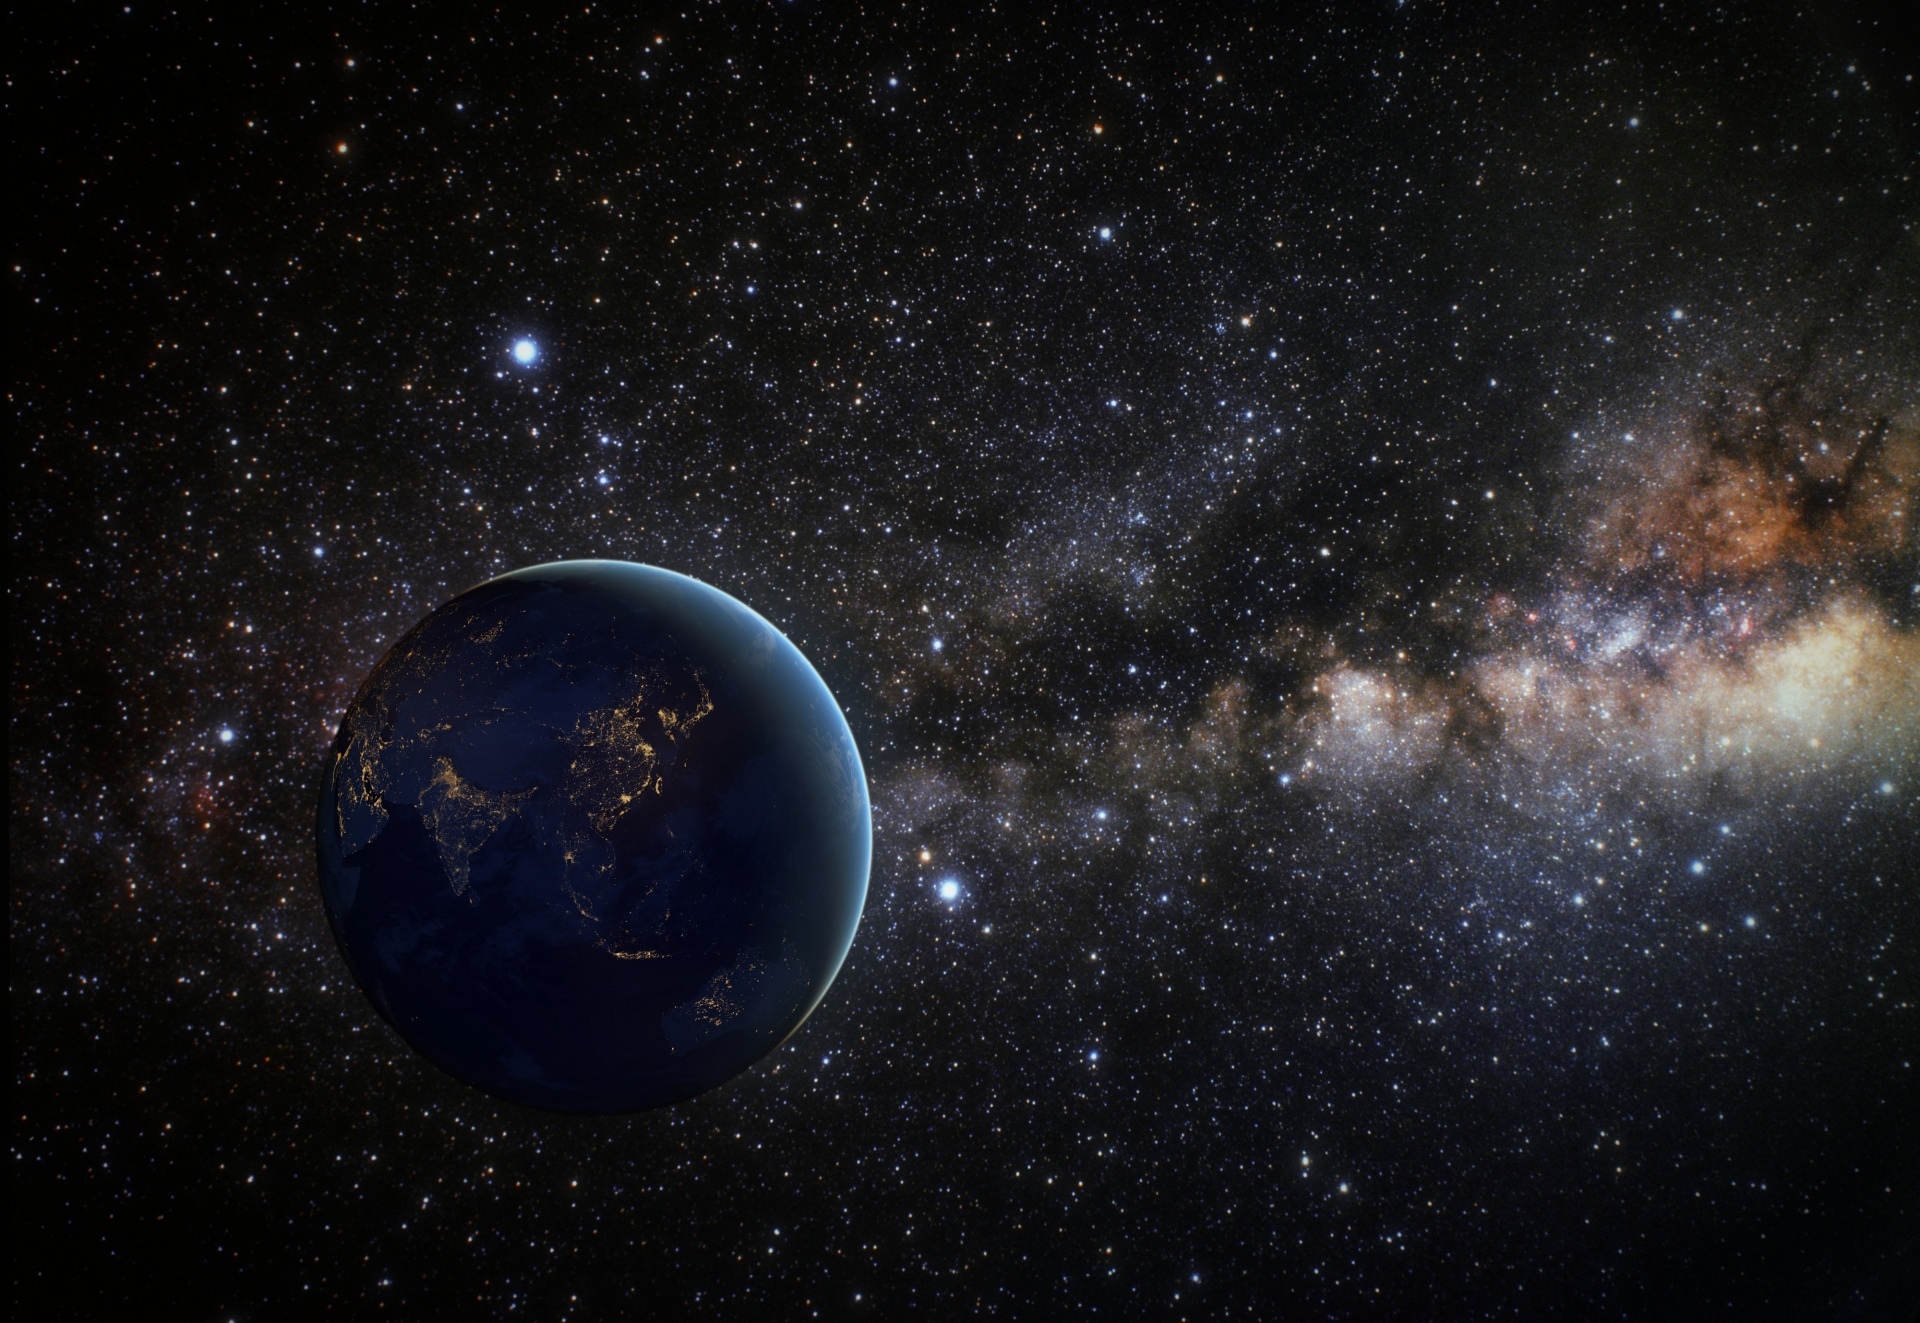
\includegraphics[width=0.5\linewidth]{figures/samples/earth-in-space.jpg}
        \caption{An example of a resized figure to be equal 50\% of the defined line width. (image source \cite{pdp:23})}
        \label{ref:resized-figure}
    \end{center}
\end{figure}

\subsection{Using Subfigures}

Sometimes the figures we want to add are a collection of images instead of a single image. And we want to add all of these images under a single \verb|\begin{figure}| \verb|...| \verb|\end{figure}| environment. We do this by using \verb|\begin{subfigure}| \verb|...| \verb|\end{subfigure}| inside of the figure environment for each sub-figure. The code is self explanatory, but we should point out the use of \verb|\hfill| and \verb|~|. We use \verb|\hfill| to tell {\LaTeX} to fill the rest of the horizantal space and start from the begining of the line. Thus, you see we use it between Figure-\ref{fig:sub-top-rigth} and Figure-\ref{fig:sub-bottom-left}. And the symbol \verb|~| is used to tell {\LaTeX} that we have two distinct objects. Therefore, {\LaTeX} will know that one has ended and another one is about to start. The symbol can be seen in use between Figure-\ref{fig:sub-top-left} and Figure-\ref{fig:sub-top-rigth}. Also, between Figure-\ref{fig:sub-bottom-left} and Figure-\ref{fig:sub-bottom-right}. 

Another thing we should note is the sizing configuration. With each \verb|\begin{subfigure}| \verb|...| \verb|\end{subfigure}| environment you can see that we say its size is \verb|{.45\textwidth}|, which means 45\% of the line width size. However, also for each \verb|\includegraphics| command we say \verb|[width=\linewidth]| without any percentage value, because the line width value now is already minimized to 45\% of its original size as long as we are withing the \verb|\begin{subfigure}| \verb|...| \verb|\end{subfigure}| environment we defined. 

\begin{figure}[H]
    \centering
    \begin{subfigure}{.45\textwidth}
        \centering
        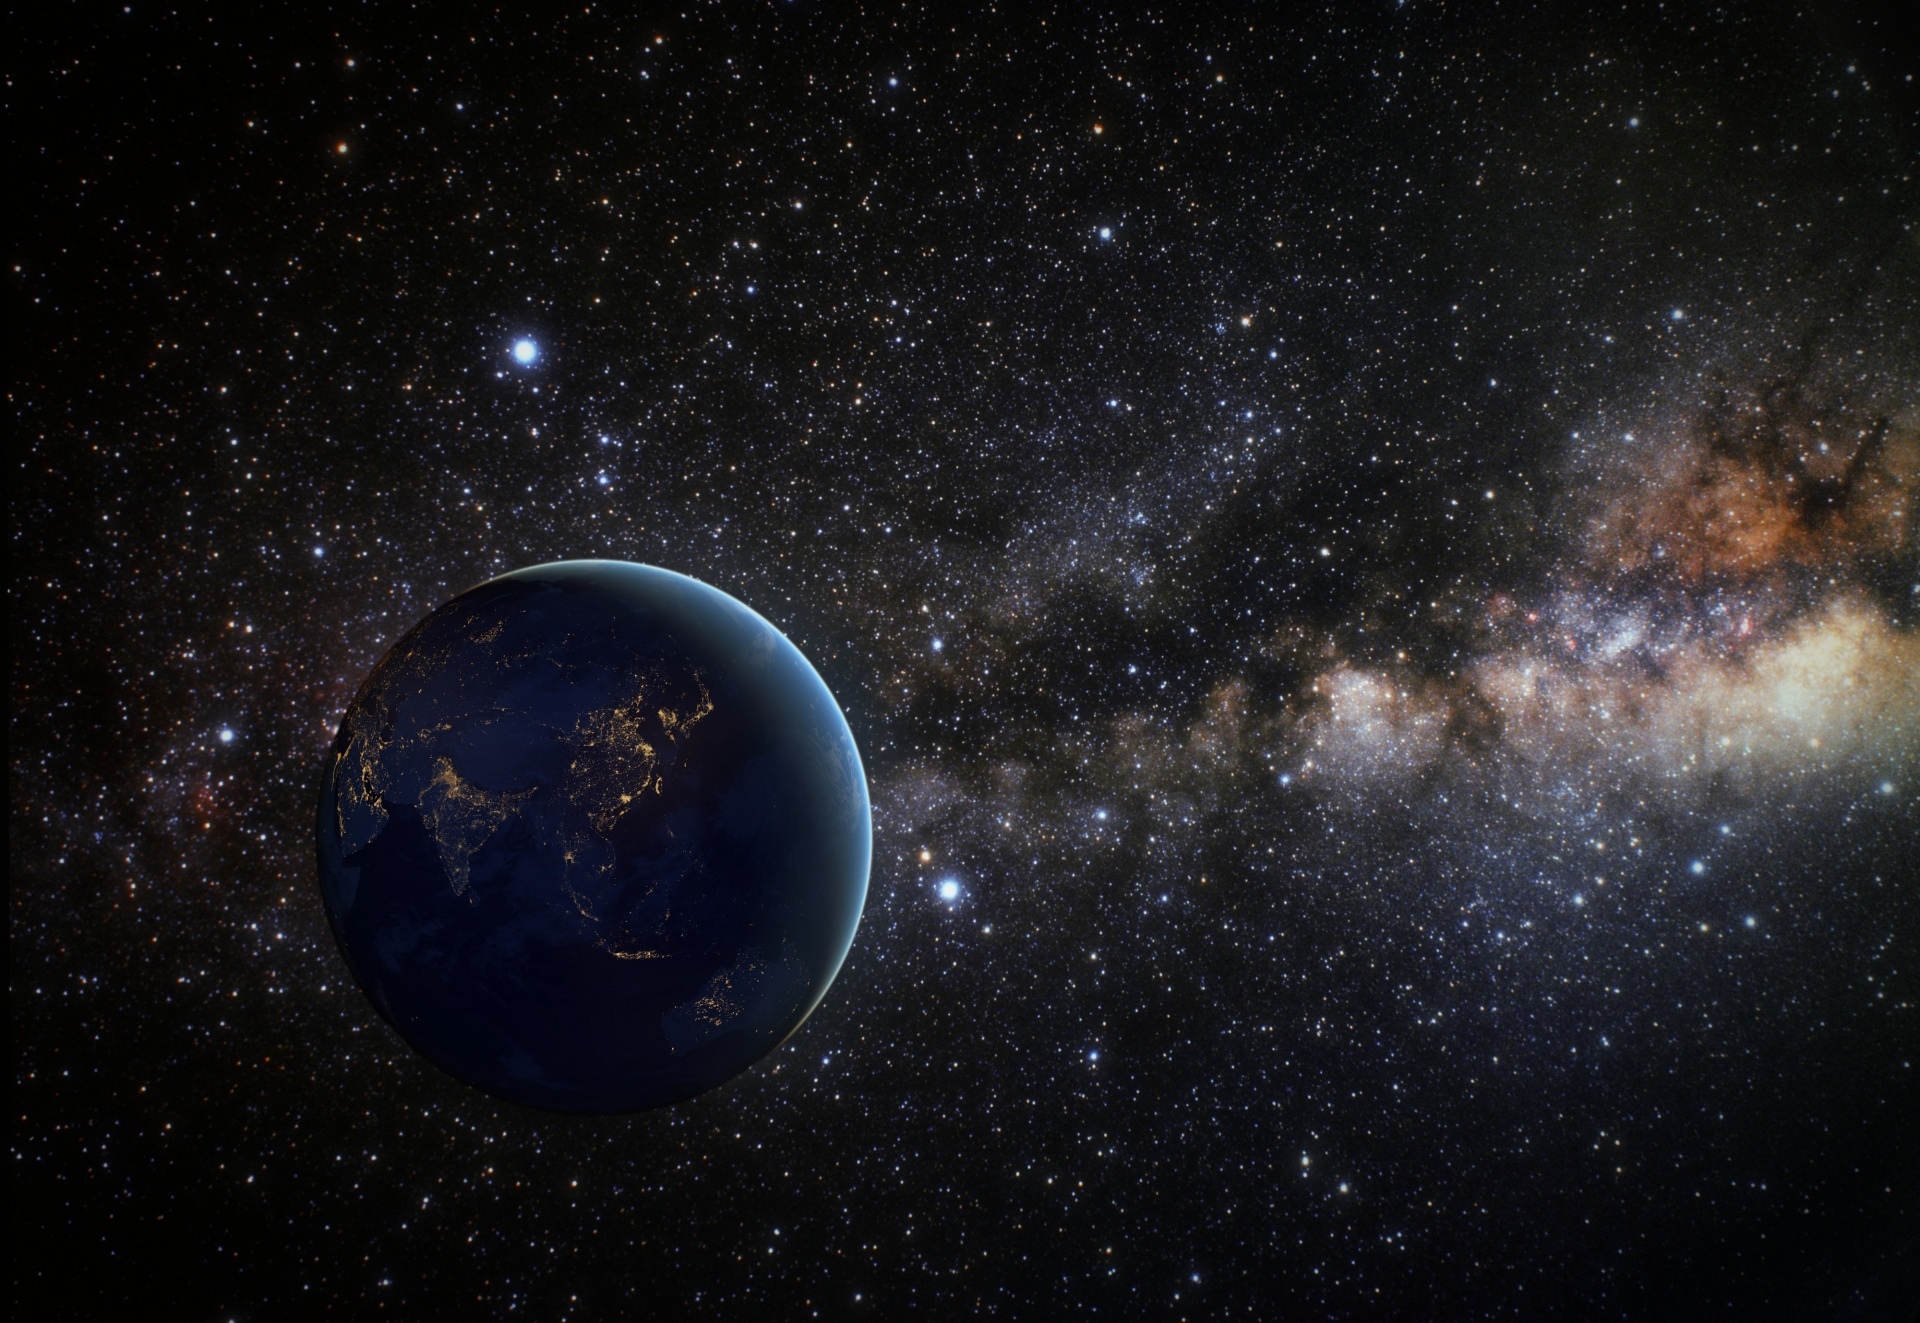
\includegraphics[width=\linewidth]{figures/samples/earth-in-space.jpg}
        \caption{Top-left sub-figure}
        \label{fig:sub-top-left}
    \end{subfigure}
    ~
    \begin{subfigure}{.45\textwidth}
        \centering
        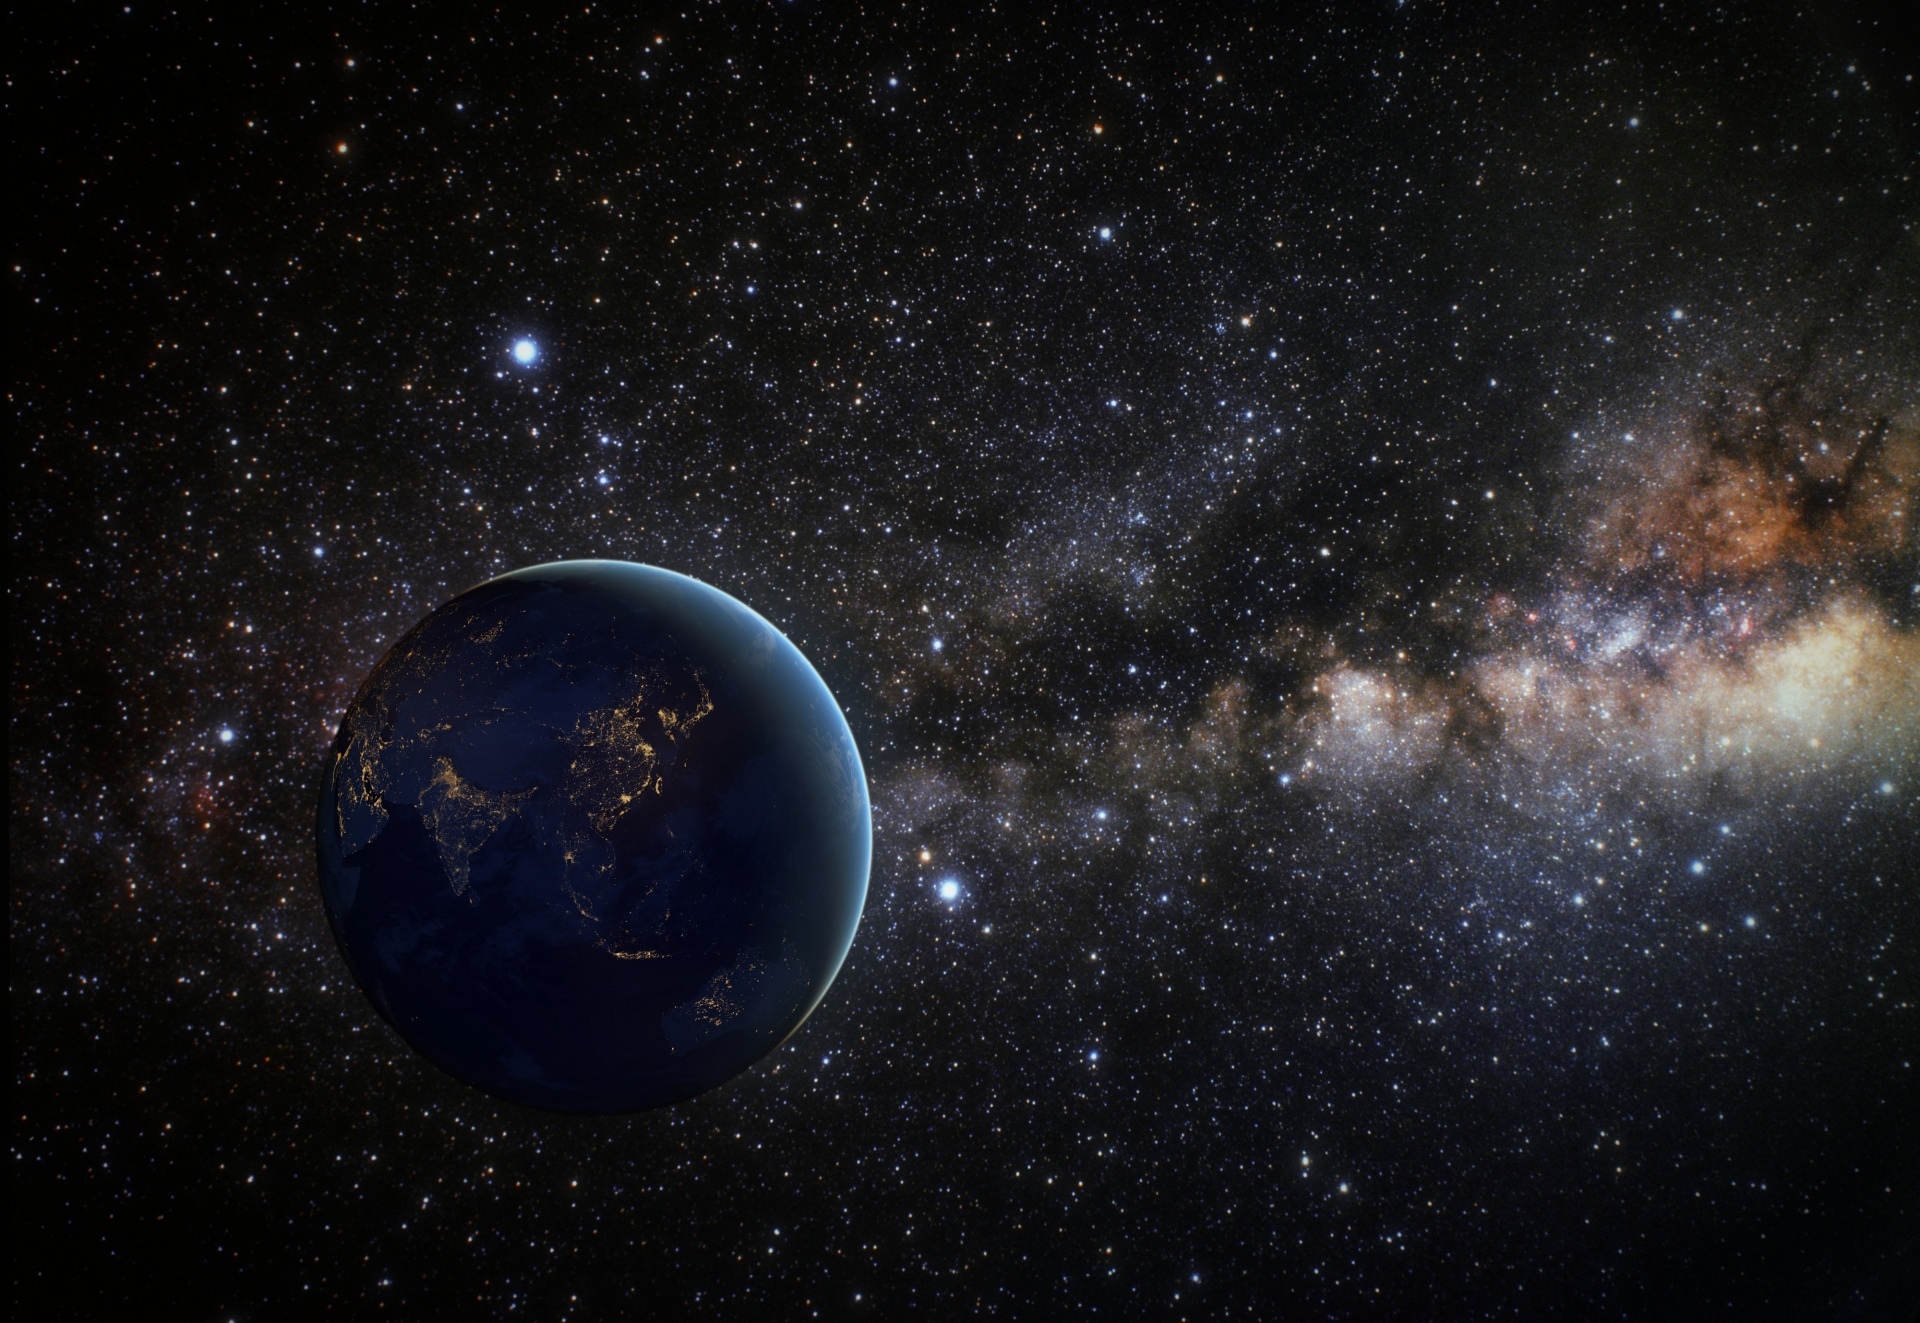
\includegraphics[width=\linewidth]{figures/samples/earth-in-space.jpg}
        \caption{Top-right sub-figure}
        \label{fig:sub-top-rigth}
    \end{subfigure}
    \hfill
    \begin{subfigure}{.45\textwidth}
        \centering
        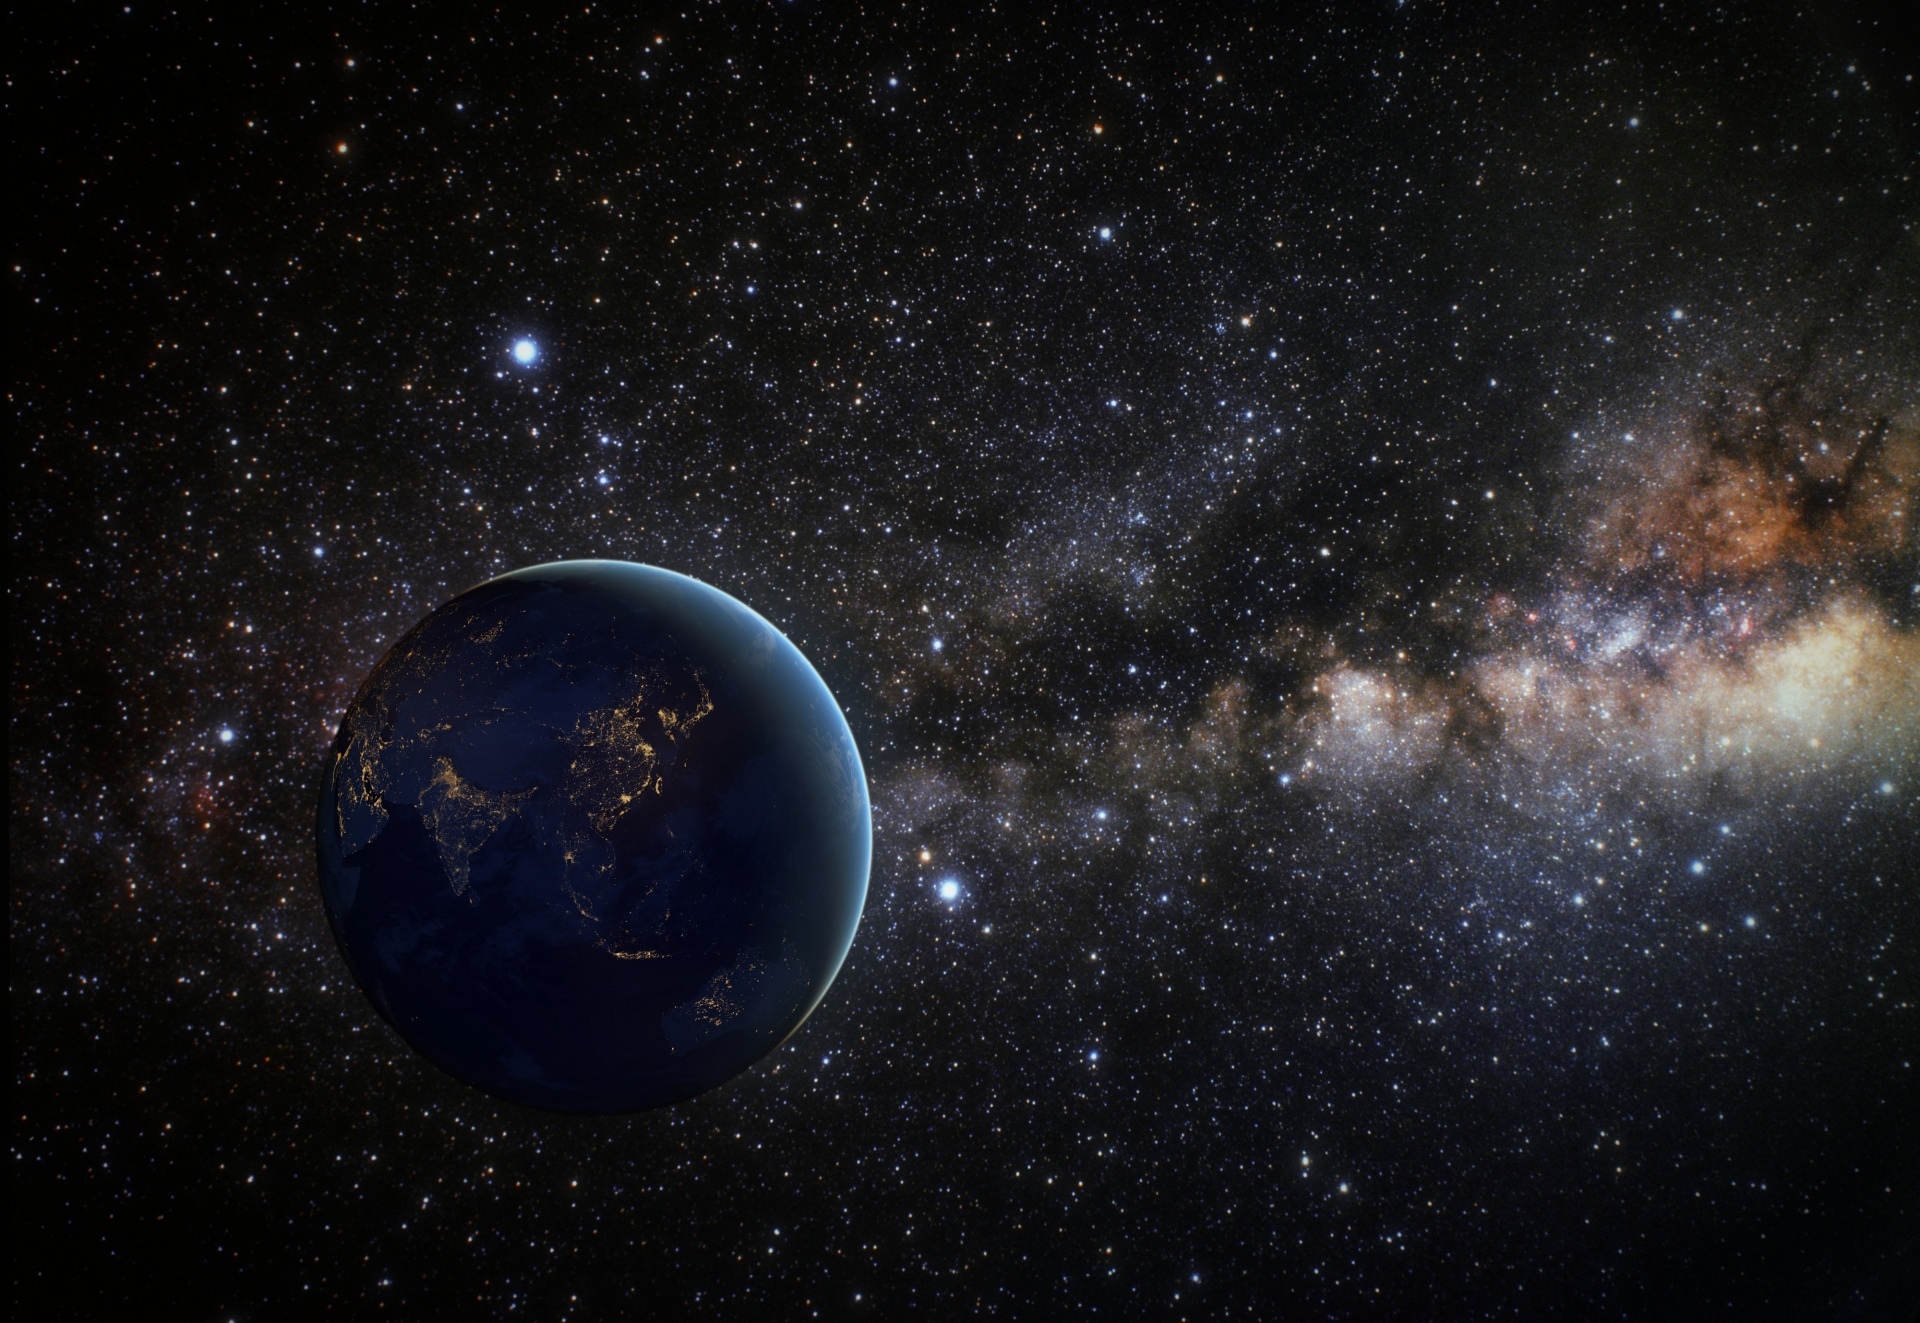
\includegraphics[width=\linewidth]{figures/samples/earth-in-space.jpg}
        \caption{Bottom-left sub-figure}
        \label{fig:sub-bottom-left}
    \end{subfigure}
    ~
    \begin{subfigure}{.45\textwidth}
        \centering
        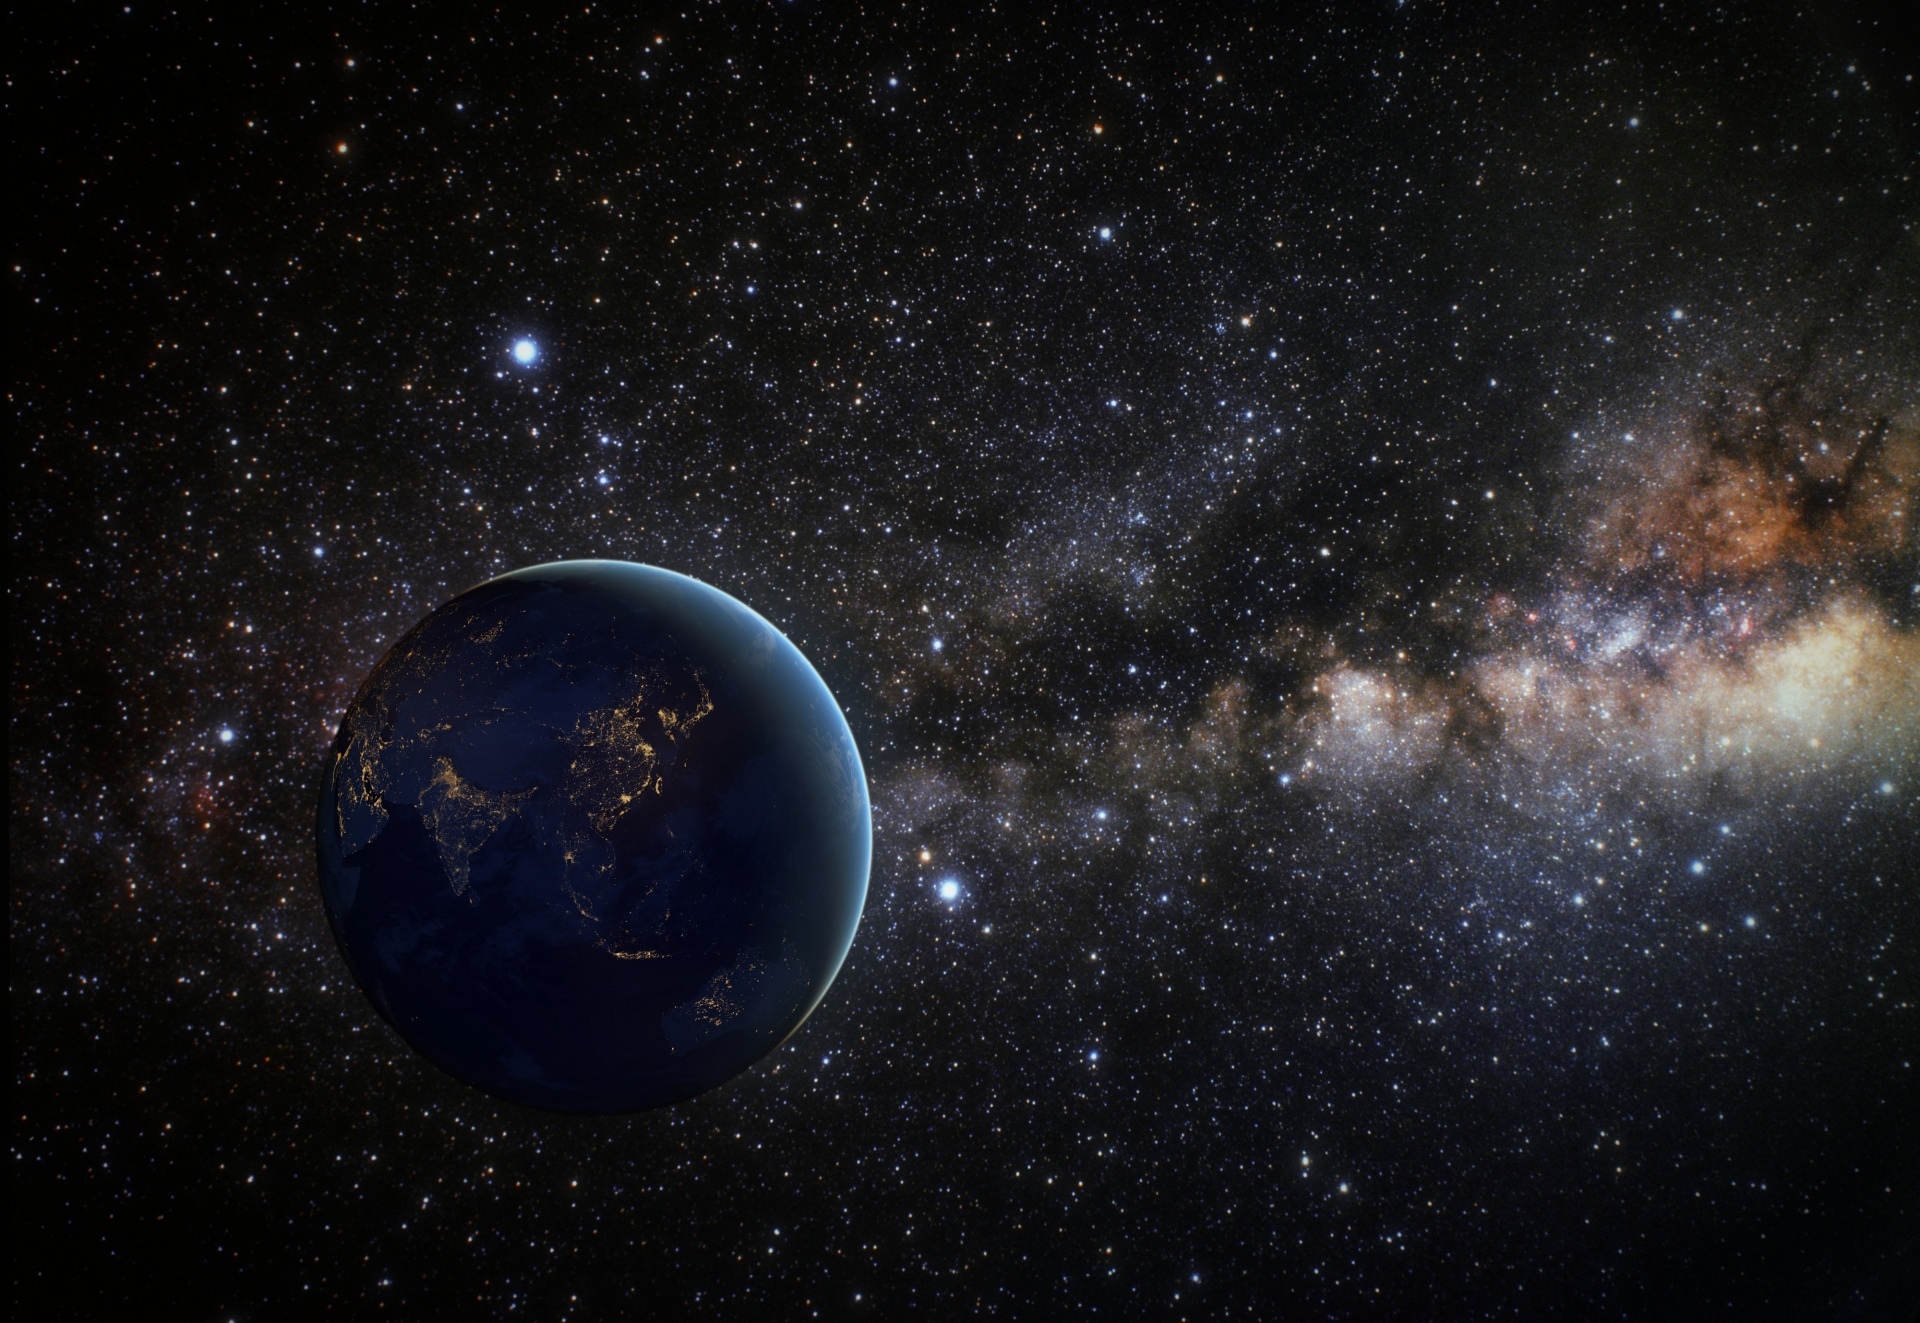
\includegraphics[width=\linewidth]{figures/samples/earth-in-space.jpg}
        \caption{Bottom-right sub-figure}
        \label{fig:sub-bottom-right}
    \end{subfigure}
    \caption{A figure that has many sub-figures placed as a grid. (image source \cite{pdp:23})}
    \label{fig:main-label-for-subfigures}
\end{figure}


\subsection{Rotated Figure}

Sometimes we need to make a figure show in a side way position. For that we need to use a special floating environment named  \verb|\begin{sidewaysfigure}| \verb|...| \verb|\end{sidewaysfigure}|. Figure-\ref{fig:rotated-figure} show an example of the use of the \verb|sidewaysfigure| environment. 

\clearpage
\begin{sidewaysfigure}
    \begin{center}
    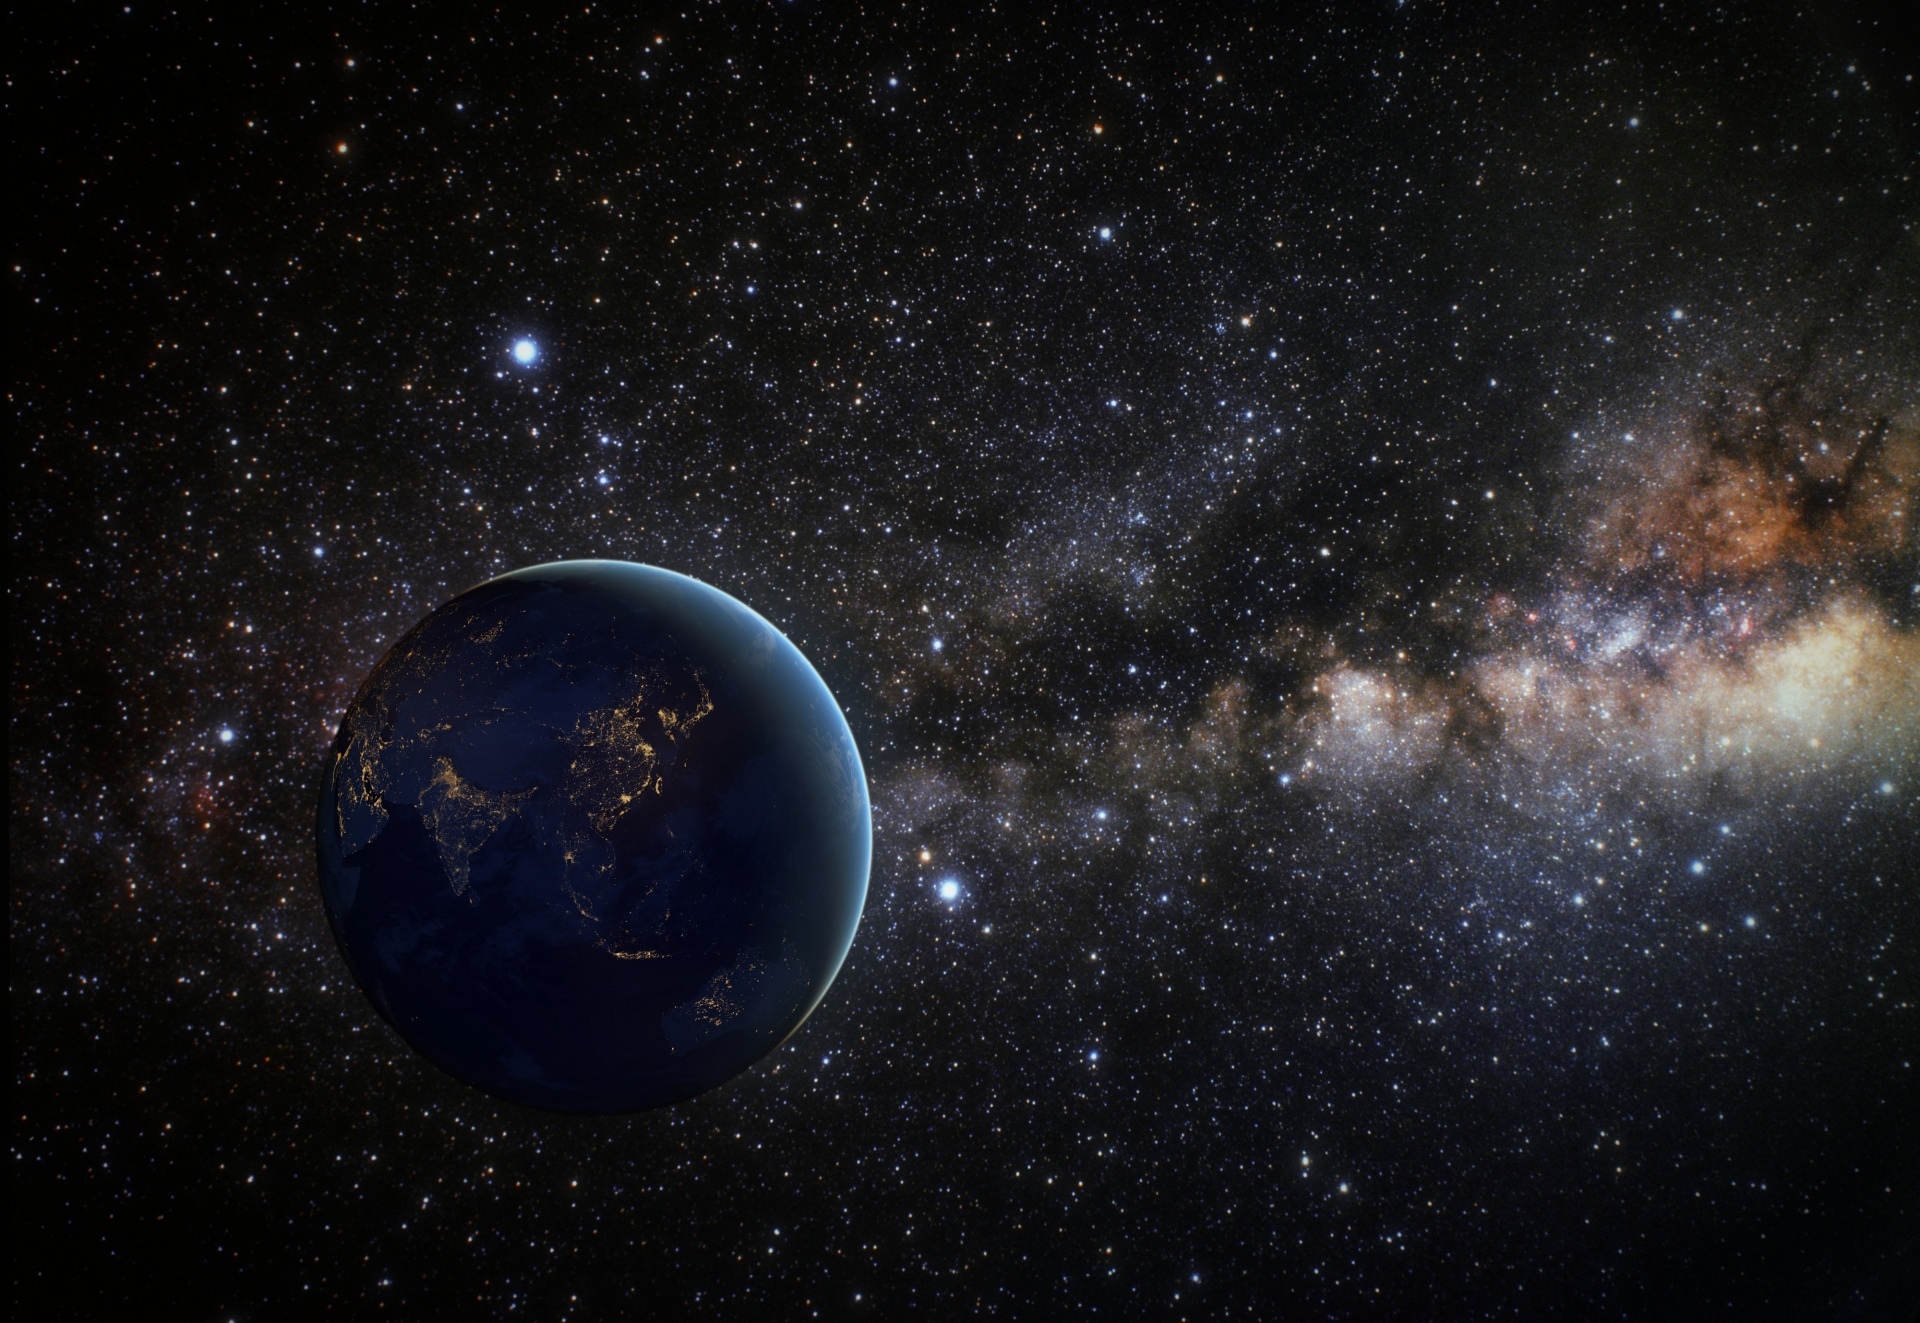
\includegraphics[width=0.6\textwidth]{figures/samples/earth-in-space.jpg}
    \caption{A rotated figure. (image source \cite{pdp:23})}
    \label{fig:rotated-figure}
    \end{center}
\end{sidewaysfigure}
\clearpage

\subsection{Using PNG vs. PDF Images}

With the figure environment, you can either PNG/JPG or PDF based images. You should use what you have, but whenever possible, we recommend you use a PDF based image/chart. The reason a PDF is better than PNG (or any other fixed imaged type), is that the resolution with a PDF scales much better than other types. Take Figure-\ref{ref:pdf-based} as an example and compare it to the image in Figure-\ref{ref:png-based}. If you zoom-in into the PDF based figure you will see it scales better than the PNG based image. 


\begin{figure}[H]
    \begin{center}
        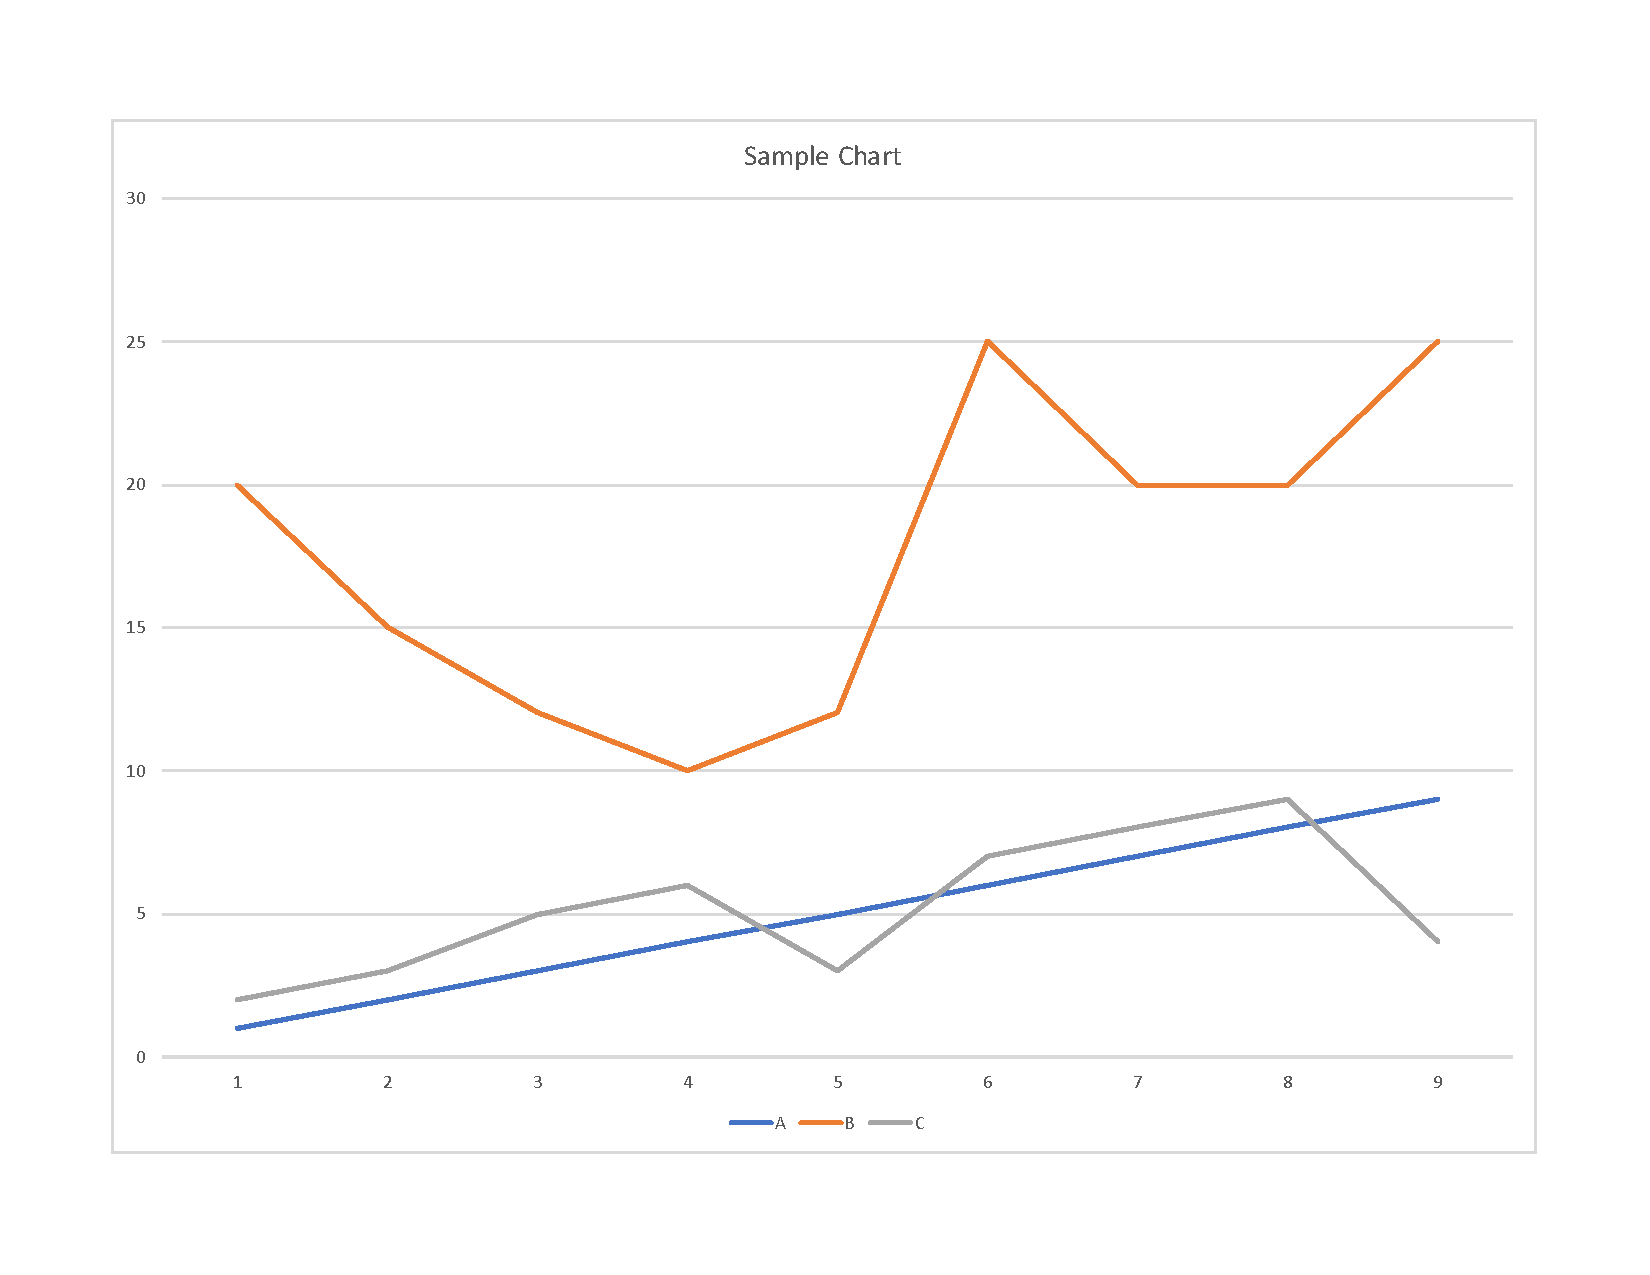
\includegraphics[width=0.5\linewidth]{figures/samples/pdf-sample.pdf}
        \caption{A PDF based figure.}
        \label{ref:pdf-based}
    \end{center}
\end{figure}

\begin{figure}[H]
    \begin{center}
        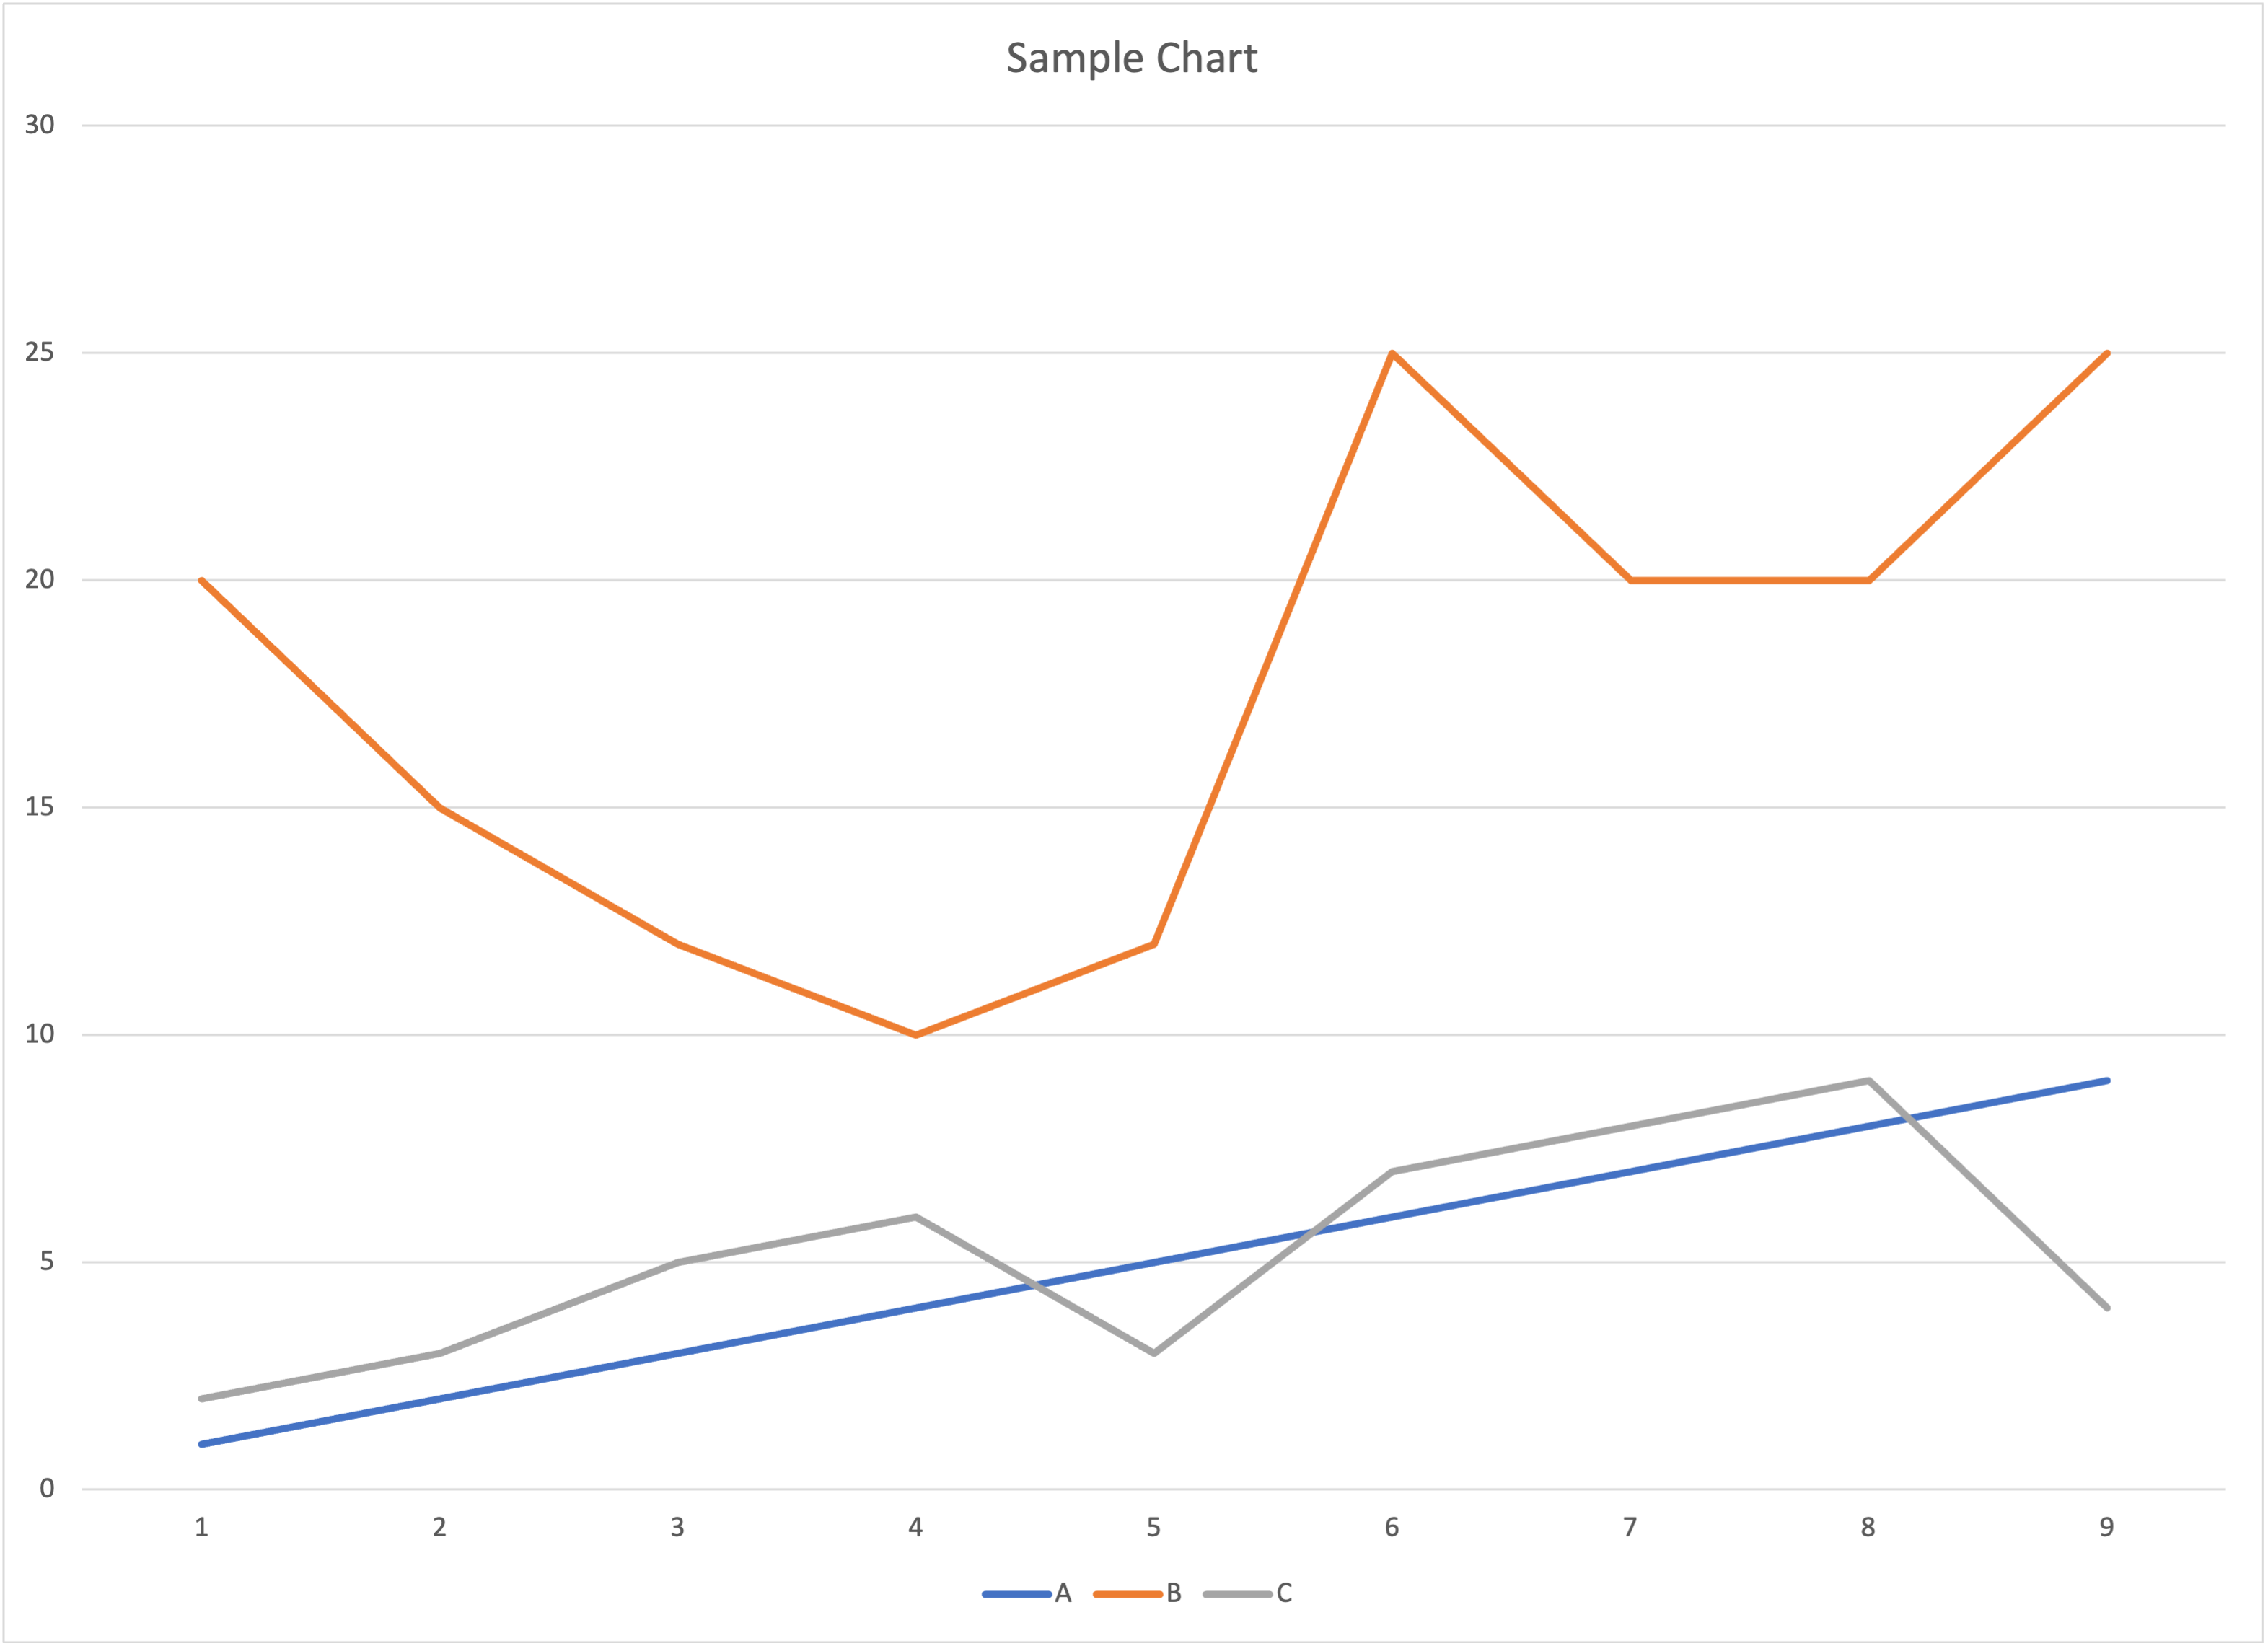
\includegraphics[width=0.5\linewidth]{figures/samples/png-sample.png}
        \caption{A PNG based figure.}
        \label{ref:png-based}
    \end{center}
\end{figure}



% ============================================================
\section{Dealing with Tables}
\label{sec:dealing_with_tables}
% ============================================================

Tables with {\LaTeX} are highly customizable. You can achieve any layout you want as you will see in this section. However, tables also can be intimidating the first time you use them with {\LaTeX}. Therefore, we recommend you to use {\LaTeX} table building tools to start with the main body of the table then you customize it as you need. There are different tools out there, but a popular one could be \href{https://www.tablesgenerator.com/}{https://www.tablesgenerator.com/}.

Next, we share few common tables layouts broken by sub-sections as given below.

\subsection{Simple Table}

The example given in Table-\ref{tab:simple-table} is for the basic table layout. The table does not have any boarders. All it has is just content broken by 3 columns and 4 rows. The table environment is given by \verb|\begin{table}| \verb|...| \verb|\end{table}|. And the content of the table itself is wrapped inside the \verb|\begin{tabular}| \verb|...| \verb|\end{tabular}| environment. Notice that after the \verb|\begin{tabular}| we add \verb|{lll}|, for which each letter correspond to the a column in the table and the letter \emph{l} in this case means align text to the left for each column.

\begin{table}[H]
    \centering
    \begin{tabular}{lll}
        Course Title      & Grade & Level \\
        Operating System  & A     & 5     \\
        Data Structure    & B     & 4     \\
        Computer Networks & A     & 7     \\
    \end{tabular}
    \caption{Simple table without boarders and text align to the left.}
    \label{tab:simple-table}
\end{table}


\subsection{All Boarders Table}

The table in this section (Table-\ref{tab:simple-table-all-boarders}) is exactly same as the table in the previous section (Table-\ref{tab:simple-table}). However, this time we add all boarders. For vertical lines, we updated the columns \verb|{lll}| by adding the symbol \emph{|} between all the letters which says we need a border line to the left of the first column, the right of the first column and so on. Also, we used \verb|\hline| at the end of each row which say draw a horizontal line. With these changes only we have full boarders. 

\begin{table}[H]
    \centering
    \begin{tabular}{|l|l|l|}
        \hline
        Course Title      & Grade & Level \\ \hline
        Operating System  & A     & 5     \\ \hline
        Data Structure    & B     & 4     \\ \hline
        Computer Networks & A     & 7     \\ \hline
    \end{tabular}
    \caption{Simple table with all boarders and text align to the left.}
    \label{tab:simple-table-all-boarders}
\end{table}


\subsection{A Beautified Version of the Simple Table}

Now you should be able to understand the basic settings that you can update to change how the table looks. In Table-\ref{tab:simple-table-beautified} we show a sample of a layout that makes the table easy to read and looks acceptable. You can change the boarders and alignment however you see fit to your case. But always think about the reader and how you could make their task in reading the tables easier.

\begin{table}[H]
    \centering
    \begin{tabular}{lll}
        \hline\hline
        Course Title      & Grade & Level \\ \hline\hline
        Operating System  & A     & 5     \\
        Data Structure    & B     & 4     \\
        Computer Networks & A     & 7     \\ \hline
    \end{tabular}
    \caption{A beautified version of the simple table.}
    \label{tab:simple-table-beautified}
\end{table}

\subsection{A Table with a Wrapped Text}


Sometimes you would have a table with a very long text in each row. The simple tables we shared previously will go beyond the page boarders as shown in Table-\ref{tab:over-boarder-table}. To make sure the table stays within the page boarder in the case of long text, you need to specify the table size. The trick can simply be by changing the alignments of the text on each column from general alignment as seen in Table-\ref{tab:over-boarder-table} (\verb|\begin{tabular}|\verb|{llll}|) to be based on the page defined margins as seen in Table-\ref{tab:wrapped-table} (\verb|\begin{tabular}| \verb|{p{0.15\textwidth}| \verb|p{0.05\textwidth}| \verb|p{0.05\textwidth}| \verb|p{0.6\textwidth}}|).

The new column definitions simply specify the space each column is allowed. Starting from the left, the first column is allowed 15\% of the text-width, the second and third columns are allowed 5\% of the text-width each, and the last column is allowed 60\% of the text-width. Given these definitions, {\LaTeX} will find a way to break the text each time it reach the allowed size limit for each column.


\begin{table}[H]
    \centering
    \begin{tabular}{llll}
        \hline\hline
        Course Title      & Grade & Level & Description \\ \hline\hline
        Operating System  & A     & 5     & Operating system course focus on the building blocks of the operating system, how can we secure them, and how to maintain a good performance for overall.\\
        Data Structure    & B     & 4     & The Data Structure course gives an overview of data structure concepts, arrays, stack, queues, trees, and graphs. Discussion of various implementations of these data objects, programming styles, and run-time representations. Course also examines algorithms for sorting, searching and some graph algorithms.\\
        Computer Networks & A     & 7     & Computer Networks course provides an introduction to computer networks, with a special focus on Internet architecture and protocols. Topics include layered network architectures, addressing, naming, forwarding, routing, communication reliability, the client-server model, web, and email protocols.\\ \hline
    \end{tabular}
    \caption{A table that does not handle long text.}
    \label{tab:over-boarder-table}
\end{table}

\begin{table}[H]
    \centering
    \begin{tabular}{p{0.15\textwidth}p{0.05\textwidth}p{0.05\textwidth}p{0.6\textwidth}}
        \hline\hline
        Course Title      & Grade & Level & Description \\ \hline\hline
        Operating System  & A     & 5     & Operating system course focus on the building blocks of the operating system, how can we secure them, and how to maintain a good performance for overall.\\
        Data Structure    & B     & 4     & The Data Structure course gives an overview of data structure concepts, arrays, stack, queues, trees, and graphs. Discussion of various implementations of these data objects, programming styles, and run-time representations. Course also examines algorithms for sorting, searching and some graph algorithms.\\
        Computer Networks & A     & 7     & Computer Networks course provides an introduction to computer networks, with a special focus on Internet architecture and protocols. Topics include layered network architectures, addressing, naming, forwarding, routing, communication reliability, the client-server model, web, and email protocols.\\ \hline
    \end{tabular}
    \caption{A table that wrapped long text by defining the table size.}
    \label{tab:wrapped-table}
\end{table}


\subsection{A Table Spanning Multiple Pages}

It is sometimes possible that you will have a table with many rows for which you cannot fit them in one page. The simple \verb|\begin{table}| \verb|...| \verb|\end{table}| environment will not help in breaking the table over multiple pages. There is a custom environment named \verb|\begin{longtable}| \verb|...| \verb|\end{longtable}| that deals with such cases. Table-\ref{tab:long-table} shows an example of a table with 51 rows. We did not specify when the table should be broken into pages. All we did is wrapped the information inside the \emph{longtable} environment with few definitions that makes reading the table easier for the reader. 

\clearpage
\begin{longtable}{|c|c|c|c|}
    \caption{A simple long-table Example}\label{tab:long-table}\\
    \hline
    \textbf{First entry} & \textbf{Second entry} & \textbf{Third entry} & \textbf{Fourth entry} \\
    \hline
    \endfirsthead
    \multicolumn{4}{c}%
    {\tablename\ \thetable\ -- \textit{Continued from previous page}} \\
    \hline
    \textbf{First entry} & \textbf{Second entry} & \textbf{Third entry} & \textbf{Fourth entry} \\
    \hline
    \endhead
    \hline \multicolumn{4}{r}{\textit{Continued on next page}} \\
    \endfoot
    \hline
    \endlastfoot
    1 & 1 & 1 & 1 \\
    2 & 2 & 2 & 2 \\
    3 & 3 & 3 & 3 \\
    4 & 4 & 4 & 4 \\
    5 & 5 & 5 & 5 \\
    6 & 6 & 6 & 6 \\
    7 & 7 & 7 & 7 \\
    8 & 8 & 8 & 8 \\
    9 & 9 & 9 & 9 \\
    10 & 10 & 10 & 10 \\
    11 & 11 & 11 & 11 \\
    12 & 12 & 12 & 12 \\
    13 & 13 & 13 & 13 \\
    14 & 14 & 14 & 14 \\
    15 & 15 & 15 & 15 \\
    16 & 16 & 16 & 16 \\
    17 & 17 & 17 & 17 \\
    18 & 18 & 18 & 18 \\
    19 & 19 & 19 & 19 \\
    20 & 20 & 20 & 20 \\
    21 & 21 & 21 & 21 \\
    22 & 22 & 22 & 22 \\
    23 & 23 & 23 & 23 \\
    24 & 24 & 24 & 24 \\
    25 & 25 & 25 & 25 \\
    26 & 26 & 26 & 26 \\
    27 & 27 & 27 & 27 \\
    28 & 28 & 28 & 28 \\
    29 & 29 & 29 & 29 \\
    30 & 30 & 30 & 30 \\
    30 & 30 & 30 & 30 \\
    31 & 31 & 31 & 31 \\
    32 & 32 & 32 & 32 \\
    33 & 33 & 33 & 33 \\
    34 & 34 & 34 & 34 \\
    35 & 35 & 35 & 35 \\
    36 & 36 & 36 & 36 \\
    37 & 37 & 37 & 37 \\
    38 & 38 & 38 & 38 \\
    39 & 39 & 39 & 39 \\
    40 & 40 & 40 & 40 \\
    41 & 41 & 41 & 41 \\
    42 & 42 & 42 & 42 \\
    43 & 43 & 43 & 43 \\
    44 & 44 & 44 & 44 \\
    45 & 45 & 45 & 45 \\
    46 & 46 & 46 & 46 \\
    47 & 47 & 47 & 47 \\
    48 & 48 & 48 & 48 \\
    49 & 49 & 49 & 49 \\
    50 & 50 & 50 & 50 \\
\end{longtable}
\clearpage

\subsection{Rotated Table}

In the case you have a large table that you want to contain in one page and the only solution is to have it in a side-way layout, then similar to figures, you can use \verb|\begin{sidewaystable}| \verb|...| \verb|\end{sidewaystable}| to put a table in a rotated layout (see Table-\ref{tab:rotated-table}). 

\clearpage
\begin{sidewaystable}
    \centering
    \begin{tabular}{lll}
        \hline\hline
        Course Title      & Grade & Level \\ \hline\hline
        Operating System  & A     & 5     \\
        Data Structure    & B     & 4     \\
        Computer Networks & A     & 7     \\ \hline
    \end{tabular}
    \caption{A simple example of a rotated table}
    \label{tab:rotated-table}
\end{sidewaystable}
\clearpage


% ============================================================
\section{Adding References}
\label{sec:adding_references}
% ============================================================

One of the essential properties of research writing or a project report is to have a well organized document in terms of references. There are two types of reference. First, references to an outside source which are called bibliography. These are the papers, books, web-pages, you have read and would like to reference. Second, you have what is called cross-references. These are references to sections, figures, tables, etc. within your document. We explain the bibliography references in Section-\ref{sub:managing_and_referencing_bibliography} and the cross-references in Section-\ref{sub:cross_referencing}.


% ------------------------------------------------------------
\subsection{Managing \& Referencing Bibliography}
\label{sub:managing_and_referencing_bibliography}
% ------------------------------------------------------------

There are different types of publications that you can read and cite. In this tutorial, we do not dive into the details of how citation should be properly used scientifically. We only show samples of different publication types and how you can use {\LaTeX} to cite them. The publication types include but not limited to the following list:

\begin{itemize}
    \item @article
    \item @book
    \item @collectedbook
    \item @conference
    \item @electronic
    \item @ieeetranbstctl
    \item @inbook
    \item @incollectedbook
    \item @incollection
    \item @injournal
    \item @inproceedings
    \item @manual
    \item @mastersthesis
    \item @misc
    \item @patent
    \item @periodical
    \item @phdthesis
    \item @preamble
    \item @proceedings
    \item @standard
    \item @string
    \item @techreport
    \item @unpublished
\end{itemize}

Regardless of the different types of publications, you first need to have a file where you keep all the references. In our case, the file is stored under the name \texttt{ref.bib}. If you open that file whether in a text-editor or a dedicated application for bibliography management (e.g., JabRef), you will get a list of publication information. 

Each publication type has some essential information that must be added to the reference entry. However, the most essential entry for {\LaTeX} to work, is the reference key. The example shown in Listing-\ref{lst:simple-listing} is for a conference paper (the type is @article) and has a reference key set to ``\texttt{Mnih:AtariRL:13}''. All the other entries are details of the reference we added. For example, the \verb|author| key has a list of all the authors who published the paper, \verb|title| stores the paper title, etc. These details can be different based on the reference type (e.g., article, book, inproceedings, etc). 

The main takeaway from Listing-\ref{lst:simple-listing} we would like to point, is the reference key\\(``\texttt{Mnih:AtariRL:13}''). This is a key that you define. We recommend following a pattern to make it easier to find references. In our case, we use the first author last name, a hint from the paper title, and then the last two digits from the year in which the reference was published. Thus, if we put the key in a cite keyword within {\LaTeX} (e.g., \verb|\cite{Mnih:AtariRL:13}|), {\LaTeX} will populate a key for it and show the reference information in the reference list \cite{Mnih:AtariRL:13} (click on the reference for it to take you to the reference information). 

\begin{lstlisting}[language=BibTex,style=mystyle,caption={Sample BibTex Reference Entry},label={lst:simple-listing}]
@article{Mnih:AtariRL:13,
    author = {Volodymyr Mnih and Koray Kavukcuoglu and David Silver and Alex Graves and Ioannis Antonoglou and Daan Wierstra and Martin A. Riedmiller},
    bibsource = {dblp computer science bibliography, https://dblp.org},
    biburl = {https://dblp.org/rec/journals/corr/MnihKSGAWR13.bib},
    date-added = {2023-03-03 17:14:11 +0300},
    date-modified = {2023-03-03 17:14:38 +0300},
    eprint = {1312.5602},
    eprinttype = {arXiv},
    journal = {CoRR},
    timestamp = {Mon, 13 Aug 2018 16:47:42 +0200},
    title = {Playing Atari with Deep Reinforcement Learning},
    url = {http://arxiv.org/abs/1312.5602},
    volume = {abs/1312.5602},
    year = {2013},
    bdsk-url-1 = {http://arxiv.org/abs/1312.5602}
}
\end{lstlisting}

\subsubsection{Citing Research Papers}

Research paper can be of different types based on where are they published. The digital-library you are using to obtain the paper should have the correct classification. Nevertheless, research papers are usually \emph{@article}, \emph{@conference}, or \emph{@inproceedings}. 

What is more important is the pieces of details that are usually shouldn't be missing. To make it easier we put these in a table (Table-\ref{tab:rp-properties}). Please note that you could have more details but the ones listed in the table are usually a MUST.

\begin{table}[H]
    \centering
    \begin{tabular}{p{0.3\textwidth}p{0.6\textwidth}}
        \hline\hline
        Attribute      & Meaning \\ \hline\hline
        cite key  & The Key you use for to cite the reference.  \\
        author    & The list of authors who published the paper as they appear in the paper.  \\
        title & The paper title.  \\
        year & The year in which this paper was published.  \\
        journal or conference & The journal or conference in which the paper was published \\
        doi & The digital identifier of an object, is the paper identifier. Note that for older papers this might not be available. \\
        url & The link to where someone can find the paper. This could be the doi itself. \\ \hline
    \end{tabular}
    \caption{Research paper essential reference properties.}
    \label{tab:rp-properties}
\end{table}

We composed a sample of well known papers to show you and example of the different citation. The first papers is for Alen Turing, one of the computer science founders. In it, Turing introduced the concept of a Turing Machine, which is a mathematical model of computers \cite{Turing:Computable:36}. Chang et al., \cite{Chang:Bigtable:08} established the foundation of the map-reduce technique that runs the internet now. 

In a different subject, Volodymyr et al., \cite{Mnih:AtariRL:13} introduced a the merge between deep learning and reinforcement learning to allow computers teach themselves how to play games. And Sutskever et al., \cite{Sutskever:SeqToSeq:14}, illustrated a translation technique using neural networks.

The four papers above are a representation of different research papers from different eras. Also, they differ in being published in journals and/or conferences. We wish that you could take a look at these sample and use them as reference for any issue you might encounter. 

\subsubsection{Citing Books}

Books are similar to research paper in almost everything except they do not require a link. Table-\ref{tab:book-properties} shows the essential properties you should have in a book reference. 

\begin{table}[H]
    \centering
    \begin{tabular}{p{0.3\textwidth}p{0.6\textwidth}}
        \hline\hline
        Attribute      & Meaning \\ \hline\hline
        cite key  & The Key you use for to cite the reference.  \\
        author & The person or persons who wrote the book. \\
        editor & The person or persons who edited the book. \\
        title & The name of the book. \\
        publisher & The publisher of the book. \\
        year & The year the book was published. \\
        isbn & The international standard book number - a unique identifier determined by the International ISBN Agency. This is not mandatory but we highly recommend adding it. \\ \hline
    \end{tabular}
    \caption{Books essential reference properties.}
    \label{tab:book-properties}
\end{table}

And example book we added is for Donald Knuth \cite{Knuth:Typesetting:86}. This is a book about {\LaTeX}. Listing-\ref{lst:book-bibtex} shows the BibTex entry we used. 

\begin{lstlisting}[language=BibTex,style=mystyle,caption={Sample BibTex Reference for A Book},label={lst:book-bibtex}]
@book{Knuth:Typesetting:86,
    author = {Donald Knuth},
    date-added = {2023-03-04 00:49:21 +0300},
    date-modified = {2023-03-04 00:53:48 +0300},
    publisher = {Addison-Wesley },
    title = {Computers and Typesetting},
    volume = {A},
    isbn= {978-0201734164},
    year = {1986}
}
\end{lstlisting}

\subsubsection{Citing Web-Pages}

Web pages are another type of references that you might add. An essential different in citing web pages is to indicate when did you visit the web pages. Because web pages are subject to change, you need to record when did you visit the page and obtained the information you rely on. 

Another difference when dealing with webpages is that they do not have an explicit type in the BibTex referencing system. Most commonly, people use the type \emph{@misc} to add a reference to a webpage. Table-\ref{tab:webpage-properties} shows the essential properties you have to add when citing a webpage. 

\begin{table}[H]
    \centering
    \begin{tabular}{p{0.3\textwidth}p{0.6\textwidth}}
        \hline\hline
        Attribute      & Meaning \\ \hline\hline
        cite key  & The Key you use for to cite the reference.  \\
        author & The person or persons who published the web page. This sometimes might be difficult to find if the web page is owned by an organization. \\
        title & The title of the web page. \\
        howpublished & How was this misc reference publish? For websites we add the webpage url. \\
        note & To add the date you accessed the webpage. \\ \hline
    \end{tabular}
    \caption{Webpage essential reference properties.}
    \label{tab:webpage-properties}
\end{table}

As an example, we used our college webpage \cite{coc:23} as a reference. The entry used for the citation used is given in Listing-\ref{lst:webpage-bibtex}.

\begin{lstlisting}[language=BibTex,style=mystyle,caption={Sample BibTex Reference for A Webpage},label={lst:webpage-bibtex}]
@misc{coc:23,
    author = {Qassim University},
    date-modified = {2023-03-04 01:12:47 +0300},
    note = {Accessed: 2023-03-04},
    title = {College of Computer at Qassim University},
    url = {https://coc.qu.edu.sa/},
    bdsk-url-1 = {https://coc.qu.edu.sa/}
}
\end{lstlisting}

% ------------------------------------------------------------
\subsection{Cross Referencing}
\label{sub:cross_referencing}
% ------------------------------------------------------------

Cross-referencing is much easier than referencing bibliography. You only need two things.

\begin{enumerate}
    \item Add a label to any part in the document you want to reference. Labels are easily added by using the keyword \verb|\label{your_key}|.
    \item Reference the label wherever you need to by using the keyword \verb|\ref{your_key}|.
\end{enumerate}

Here are some cross-references that you can test.

\begin{itemize}
    \item This is a reference to Section-\ref{sec:using_lists} where we talked about how to use lists. 
    \item This is a reference to Figure-\ref{fig:main-label-for-subfigures} where we showed how to use sub-figures. 
    \item This is a reference to Table-\ref{tab:simple-table-beautified} where we showed a simple table example.
\end{itemize}


% ============================================================
\section{Mathematical Mode}
\label{sec:mathematical_mode}
% ============================================================

One of the well known strengths of {\LaTeX} is the ease and comprehensibility of writing mathematical notations. In this section we show the two cases of writing in mathematical mode. (In line as shown in Section-\ref{sub:using_mathematical_notations} and equations as shown in Section-\ref{sub:writing_mathematical_equations}).

Please note that we do not cover all the possible symbols and math forms in this section. This is just a tutorial to get you started. A good reference for mathematical writing can be found in \href{https://www1.cmc.edu/pages/faculty/aaksoy/latex/latexthree.html}{https://www1.cmc.edu/pages/faculty/aaksoy/latex/latexthree.html}.


% ------------------------------------------------------------
\subsection{Using Mathematical Notations}
\label{sub:using_mathematical_notations}
% ------------------------------------------------------------

Writing mathematical notation inline with {\LaTeX} require you to wrap the mathematical symbols between one of the following wrappers. 

\begin{itemize}
    \item \verb|\( ... \)|
    \item \verb|$ ... $|
    \item \verb|\begin{math}...\end{math}|
\end{itemize}


\begin{lstlisting}[language=Tex,style=mystyle,caption={Sample Paragraph with Inline Math Equations},label={lst:inline-math}]
This is an example of an inline math equations. This first example, $\sqrt{3}$, uses dollar signs to write an equation and it shows a square root. The second example here, \(E=mc^2\), uses parentheses to write an equation and shows the mass-energy equivalence formula. The last example we show, \begin{math} P: \widehat{G} \rightarrow G \end{math}, uses {\LaTeX} math keyword to write a G with wide hat and an arrow symbol. 

Regardless of the wrapper you use the result will always be the same. 
\end{lstlisting}

The {\LaTeX} input shown in Listing-\ref{lst:inline-math} above will result in the text shown below when we typeset it. 

This is an example of an inline math equations. This first example, $\sqrt{3}$, uses dollar signs to write an equation and it shows a square root. The second example here, \(E=mc^2\), uses parentheses to write an equation and shows the mass-energy equivalence formula. The last example we show, \begin{math} P: \widehat{G} \rightarrow G \end{math}, uses {\LaTeX} math keyword to write a G with wide hat and an arrow symbol. 

Regardless of the wrapper you use the result will always be the same. 

% ------------------------------------------------------------
\subsection{Writing Mathematical Equations}
\label{sub:writing_mathematical_equations}
% ------------------------------------------------------------

The other mathematical mode is available when you want to write a stand-alone mathematical formula/equation. For stand-alone math mode, we use the wrapper \verb|\begin{equation}| \verb|...| \verb|\end{equation}|.

\begin{equation}
    \sum_{n=1}^{\infty} 2^{-n} = 1
    \label{eq:sum}
\end{equation}

\begin{equation}
    \int_{a}^{b} x^2 \,dx
    \label{eq:int}
\end{equation}

\begin{equation}
    f(x)=\frac{P(x)}{Q(x)}\quad \textrm{and}\quad \textstyle f(x)=\frac{P(x)}{Q(x)}\quad \textrm{and}\quad \scriptstyle f(x)=\frac{P(x)}{Q(x)}
    \label{eq:frac}
\end{equation}

Here are three mathematical equations samples. Note that we can reference them just like figures and tables. I.e., the equations are Equation-\ref{eq:sum}, Equation-\ref{eq:int}, and Equation-\ref{eq:frac}. 

% ============================================================
\section{Acronyms}
\label{sec:acronyms}
% ============================================================

{\LaTeX} provides a nice package that helps you manage acronyms. The package is defined in the \texttt{00-main.tex} file. All the acronyms are defined in main file (\texttt{00-main.tex}) to be accessible for all other chapters. As an example we declared the acronyms shown in Listing-\ref{lst:acronyms}. 

\begin{lstlisting}[language=Tex,style=mystyle,caption={Sample Acronyms Declarations},label={lst:acronyms}]
\DeclareAcronym{os}{
  short = OS ,
  long  = Operating System ,
  tag = abbrev
}
\DeclareAcronym{ai}{
  short = AI ,
  long  = Artificial Intelligent ,
  tag = abbrev
}
\DeclareAcronym{dm}{
  short = DM ,
  long  = Data Mining ,
  tag = abbrev
}
\DeclareAcronym{tcp}{
  short = TCP ,
  long  = Transmission Control Protocol ,
  tag = abbrev
}
\DeclareAcronym{ml}{
  short = ML ,
  long  = Machine Learning ,
  tag = abbrev
}
\DeclareAcronym{cnn}{
  short = CNN ,
  long  = Convolutional Neural Network ,
  tag = abbrev
}
\end{lstlisting}


Now that the acronyms are declared, we can easily refer to them whenever we write about them in text. Here are the acronyms we declared in use Operating Systems (\ac{os}), Artificial Intelligent (\ac{ai}), Tranmission Control Protocol (\ac{tcp}), Machine Learning (\ac{ml}), Convolutional Neural Network (\ac{cnn}), and Data Mining (\ac{dm}). 